\section{ETFW}

No servidor virtual com a imagem da \textit{ETFW} é possível configurar o serviço através do \textit{Central Management} no separador \textit{ETFW}.

No \textit{Painel principal} podemos aceder ao configurador de rede através \textit{Network setup Wizard} ou aceder à interface de \textit{Webmin} para efectuar as alterações em toda a configuração.

\begin{figure}[H]
    \begin{center}
    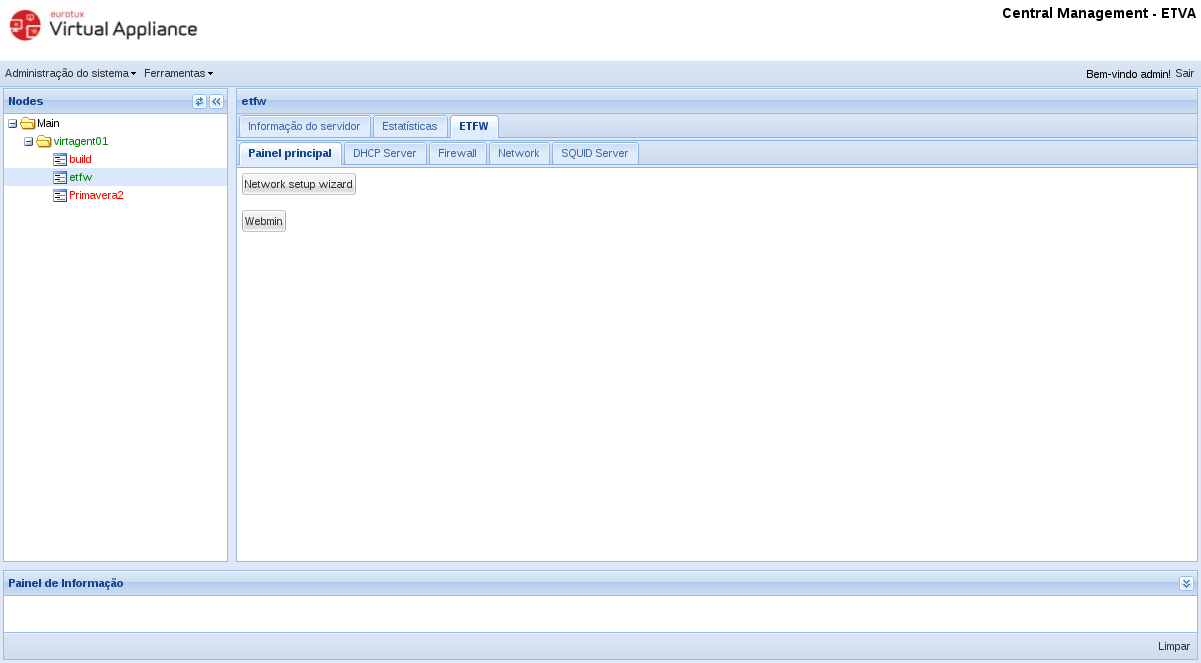
\includegraphics[scale=0.38]{screenshots/etfw/etfwmain.png}
    \caption{Painel Principal}
    \label{fig:etfwmain}
    \end{center}
\end{figure}

\subsection{Network setup Wizard}

Para configurar o módulo \textit{ETFW} de forma rápida e eficiente é disponibilizado um \textit{wizard} com configuração passo a passo.

\begin{figure}[H]
    \begin{center}
    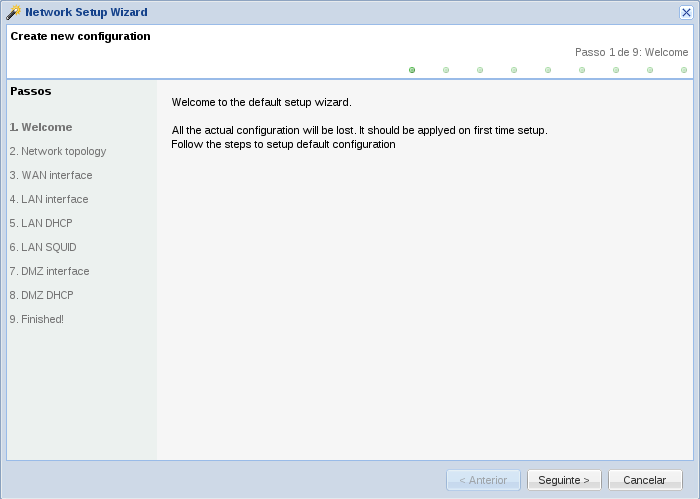
\includegraphics[scale=0.38]{screenshots/etfw/etfw_wizard_01.png}
    \caption{Boas vindas}
    \label{fig:etfw_wizard_passo1}
    \end{center}
\end{figure}

\begin{figure}[H]
    \begin{center}
    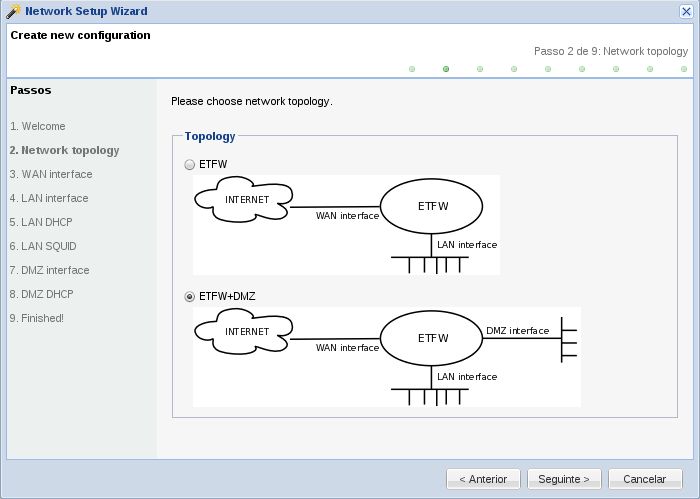
\includegraphics[scale=0.38]{screenshots/etfw/etfw_wizard_02.png}
    \caption{Configuração da topologia}
    \label{fig:etfw_wizard_passo2}
    \end{center}
\end{figure}

\begin{figure}[H]
    \begin{center}
    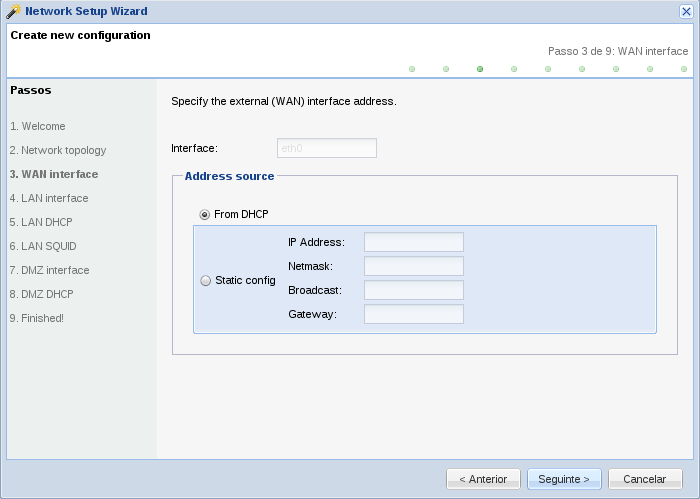
\includegraphics[scale=0.38]{screenshots/etfw/etfw_wizard_03.png}
    \caption{Configuração da interface WAN}
    \label{fig:etfw_wizard_passo3}
    \end{center}
\end{figure}

\begin{figure}[H]
    \begin{center}
    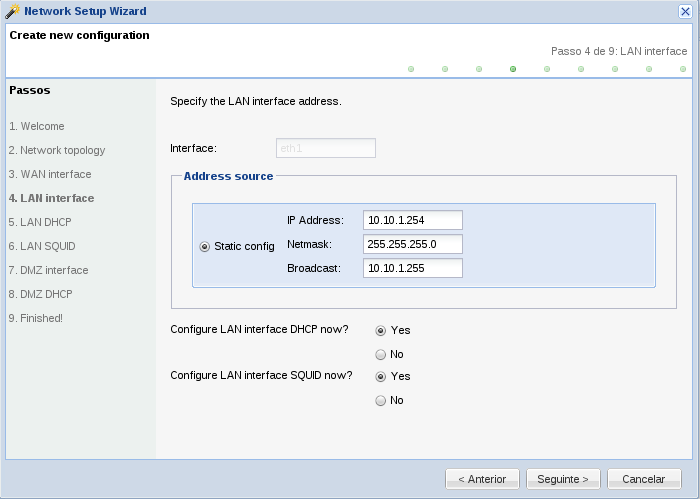
\includegraphics[scale=0.38]{screenshots/etfw/etfw_wizard_04.png}
    \caption{Configuração da interface LAN}
    \label{fig:etfw_wizard_passo4}
    \end{center}
\end{figure}

\begin{figure}[H]
    \begin{center}
    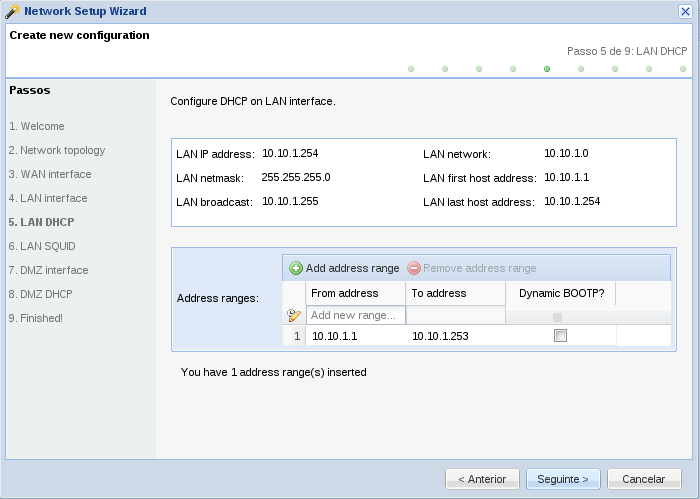
\includegraphics[scale=0.38]{screenshots/etfw/etfw_wizard_05.png}
    \caption{Configuração do serviço DHCP para a rede LAN}
    \label{fig:etfw_wizard_passo5}
    \end{center}
\end{figure}

\begin{figure}[H]
    \begin{center}
    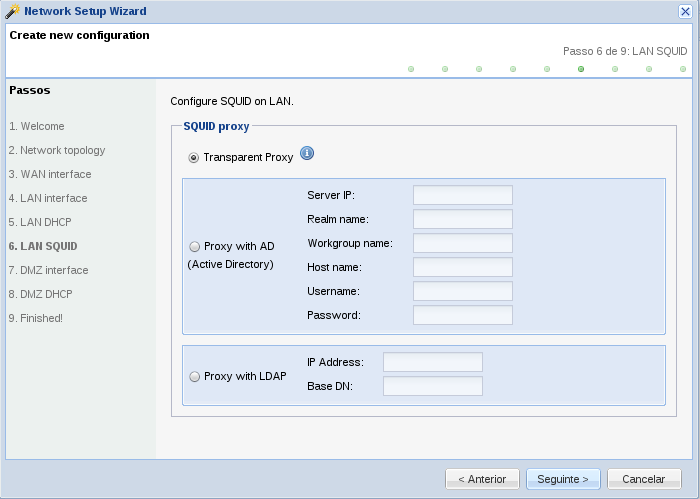
\includegraphics[scale=0.38]{screenshots/etfw/etfw_wizard_06.png}
    \caption{Configuração do proxy SQUID}
    \label{fig:etfw_wizard_passo6}
    \end{center}
\end{figure}

\begin{figure}[H]
    \begin{center}
    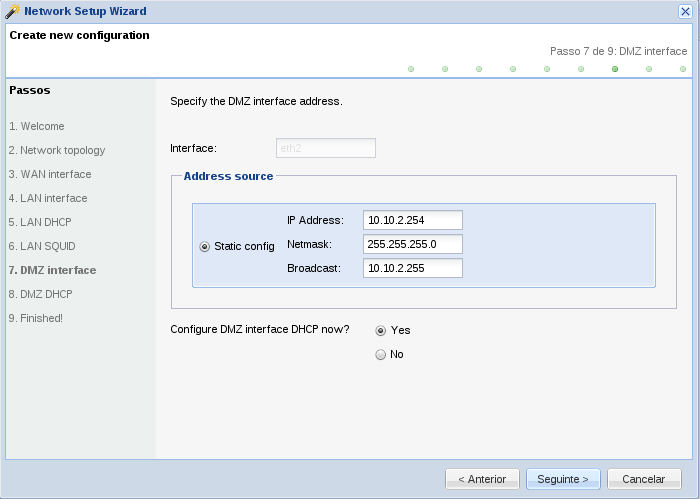
\includegraphics[scale=0.38]{screenshots/etfw/etfw_wizard_07.png}
    \caption{Configuração da interface DMZ}
    \label{fig:etfw_wizard_passo7}
    \end{center}
\end{figure}

\begin{figure}[H]
    \begin{center}
    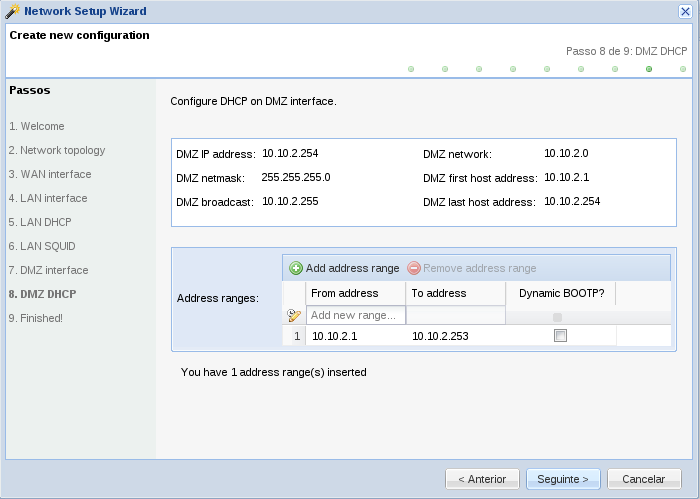
\includegraphics[scale=0.38]{screenshots/etfw/etfw_wizard_08.png}
    \caption{Configuração do serviço DHCP para a rede DMZ}
    \label{fig:etfw_wizard_passo8}
    \end{center}
\end{figure}

\begin{figure}[H]
    \begin{center}
    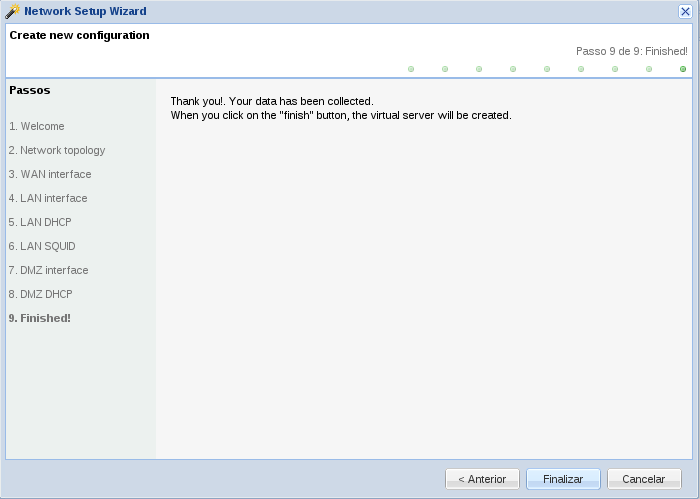
\includegraphics[scale=0.38]{screenshots/etfw/etfw_wizard_09.png}
    \caption{Finalização do processo de configuração}
    \label{fig:etfw_wizard_passo9}
    \end{center}
\end{figure}

\subsection{Edição de Rede - \textit{Network}}

Adicionalmente ao processo de configuração \textit{wizard} é possível alterar a configuração de rede manualmente.
Para isso, acedemos ao separador \textit{Network} onde temos acesso à configuração de interfaces de rede (\textit{Network interfaces}), regras de encaminhamento (\textit{Routing and gateways}), configuração de endereços (\textit{Host Addresses}) e cliente de \textit{DNS} (\textit{Hostname and DNS Client}).

\subsubsection{Interfaces de rede}

Em \textit{Interfaces de rede} podemos ver as interfaces de rede que estão configuradas actualmente e as que estão activas ao iniciar a máquina.

Ao seleccionar uma interface podemos editar os parâmetros da interface como IP, máscara de rede, endereço de \textit{broadcast} e ainda \textit{aliases} em \textit{Virtual interfaces}.
Para adicionar uma nova interface, basta seleccionar a opção \textit{add} e preencher os parâmetros da interface.

\begin{figure}[H]
    \begin{center}
    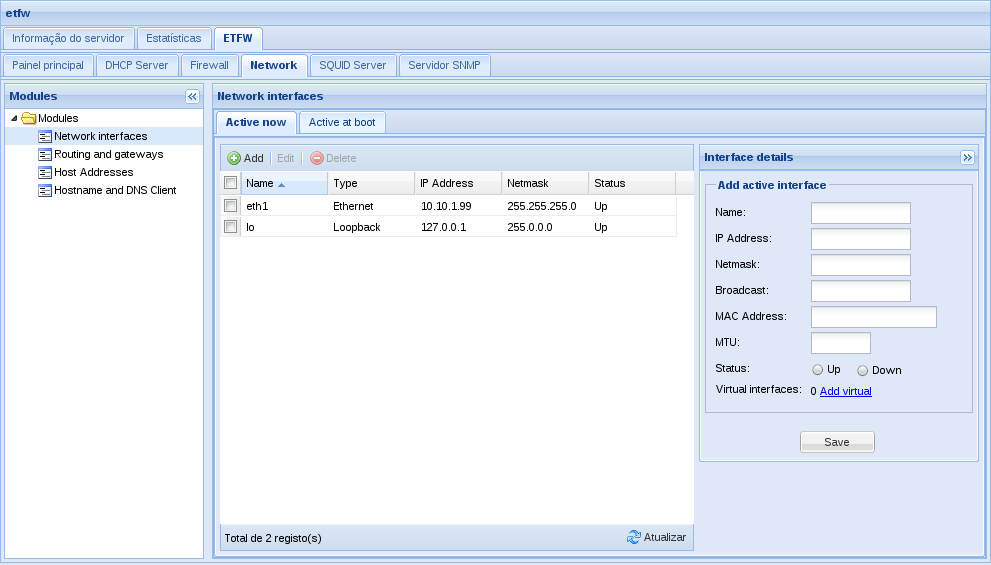
\includegraphics[scale=0.38]{screenshots/etfw/etfw_network_interfaces_01.png}
    \caption{Interfaces activas}
    \label{fig:etfw_network_interfaces_01}
    \end{center}
\end{figure}

\begin{figure}[H]
    \begin{center}
    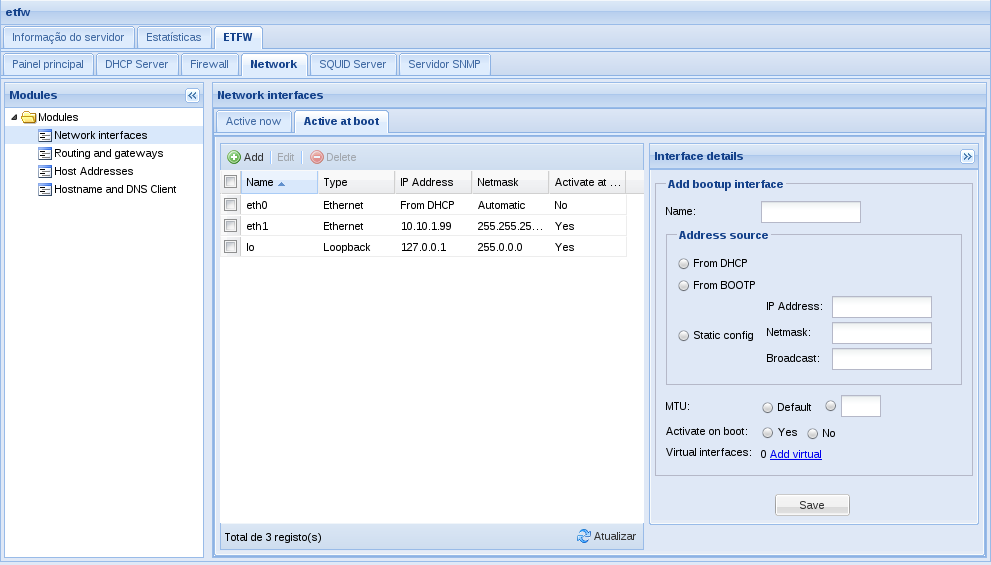
\includegraphics[scale=0.38]{screenshots/etfw/etfw_network_interfaces_02.png}
    \caption{Interfaces activas no arranque}
    \label{fig:etfw_network_interfaces_02}
    \end{center}
\end{figure}

No caso de pretender definir um alias de rede para uma interface, deverá seleccionar a interface pretendida, editar e escolher \textit{Add virtual} em \textit{Virtual interfaces}. A seguir, deverá preencher os parâmetros solicitados e guardar.

\begin{figure}[H]
    \begin{center}
    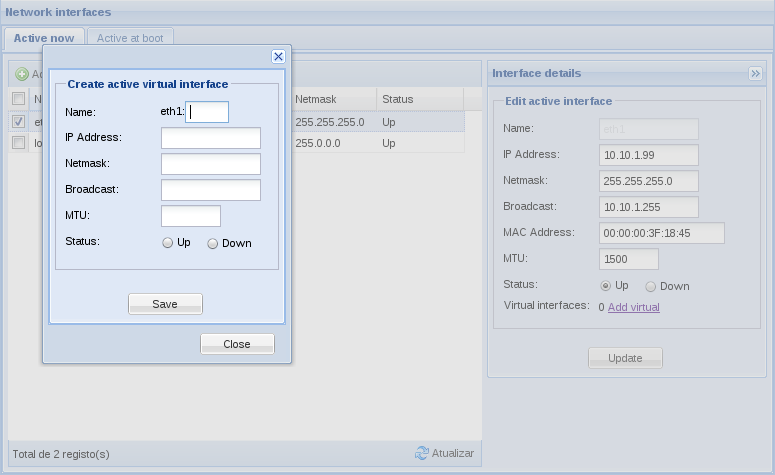
\includegraphics[scale=0.38]{screenshots/etfw/etfw_network_interfaces_03.png}
    \caption{Alias interface}
    \label{fig:etfw_network_interfaces_02}
    \end{center}
\end{figure}

\begin{figure}[H]
    \begin{center}
    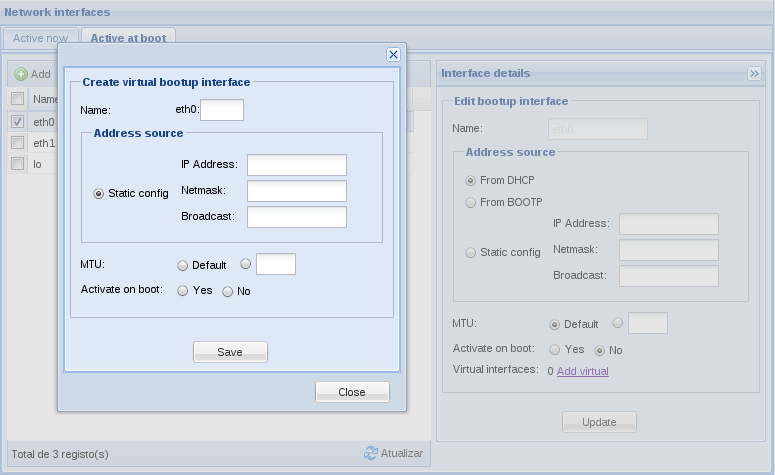
\includegraphics[scale=0.38]{screenshots/etfw/etfw_network_interfaces_04.png}
    \caption{Alias interface activa no arranque}
    \label{fig:etfw_network_interfaces_02}
    \end{center}
\end{figure}

\subsubsection{Routing and gateways}

Em \textit{Routing and gateways} podemos consultar as regras de encaminhamento activas e remove ou adicionar novas regras.
É possível também definir as regras de encaminhamento que são definidas no arranque.

\begin{figure}[H]
    \begin{center}
    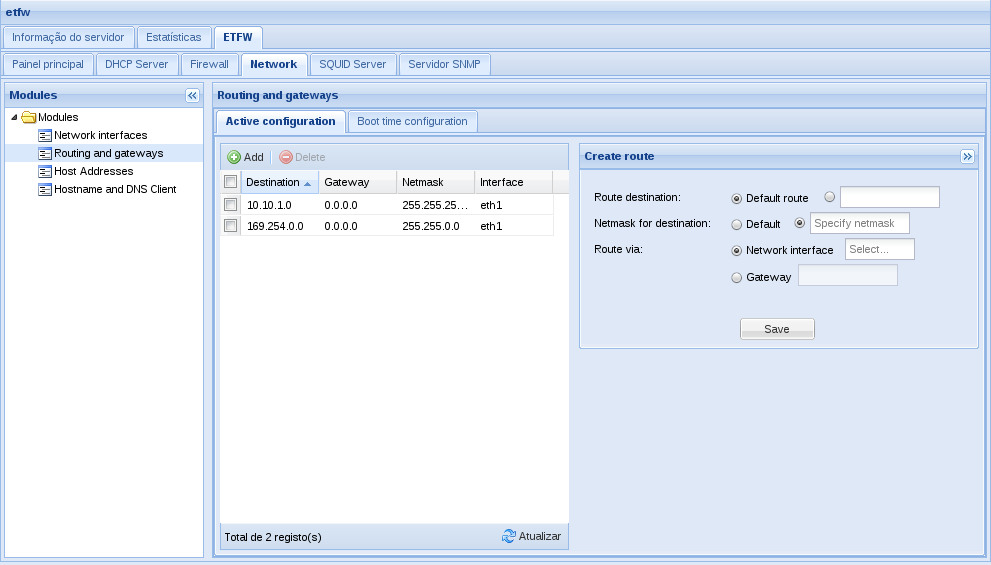
\includegraphics[scale=0.38]{screenshots/etfw/etfw_network_routing_01.png}
    \caption{Regras de encaminhamento activas}
    \label{fig:etfw_network_routing_01}
    \end{center}
\end{figure}

Para criar uma regra de encaminhamento, escolhemos a opção \textit{add} e definimos os parâmetros da rota: 

\begin{itemize}
    \item \textit{Route destination} - Destino da rota de encaminhamento, em que pode ser \textit{default}, endereço IP destino ou endereço de rede;
    \item \textit{Netmask for destination} - Máscara de rede para a rota de destino;
    \item \textit{Route via} - \textit{Gateway} ou interface de rede de saída da rota.
\end{itemize}

\begin{figure}[H]
    \begin{center}
    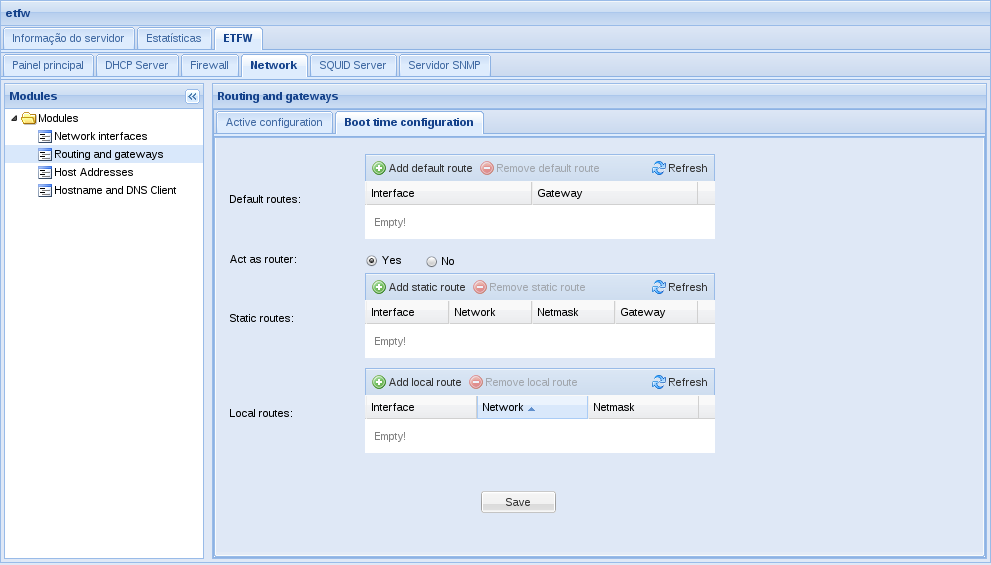
\includegraphics[scale=0.38]{screenshots/etfw/etfw_network_routing_02.png}
    \caption{Regras de encaminhamento definidas no arranque}
    \label{fig:etfw_network_routing_02}
    \end{center}
\end{figure}

Nas regras de encaminhamento definidas no arranque podemos configurar o conjunto de regras dos seguintes tipos:

\begin{itemize}
    \item \textit{Default routes} - para definir a \textit{gateway} por omissão;
    \item \textit{Static routes} - rotas estáticas para outras redes e/ou máquinas;
    \item \textit{Local routes} - rotas locais onde são especificados endereços de IP, máscara de rede e interface de cada rota.
\end{itemize}

\subsubsection{Host Addresses}

Em \textit{Host Addresses} é possível definir os nomes fixos e locais associados aos endereços de IP, de forma a diminuir o tempo de resposta na resolução de nomes.

\begin{figure}[H]
    \begin{center}
    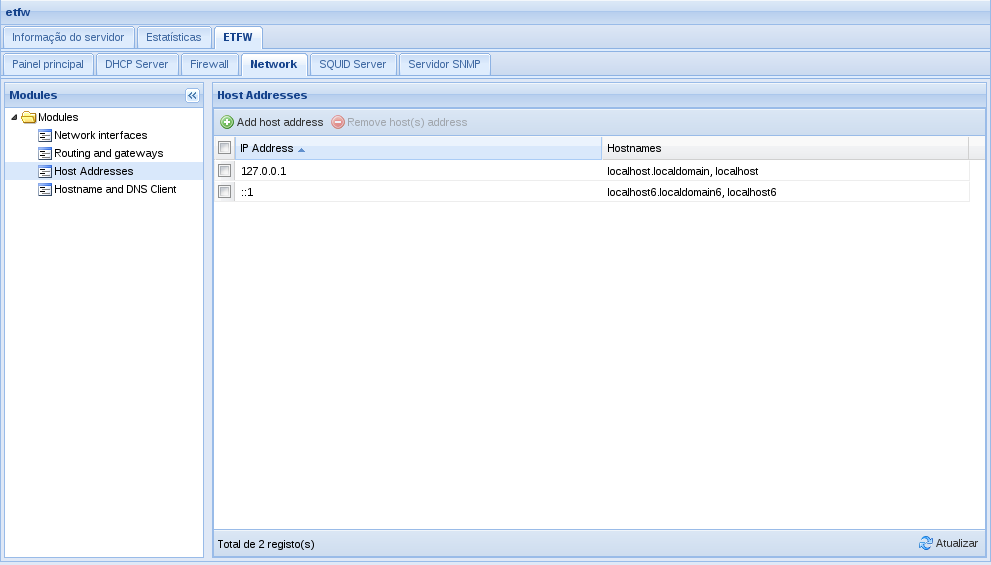
\includegraphics[scale=0.38]{screenshots/etfw/etfw_network_hostaddresses_01.png}
    \caption{Configuração de endereços}
    \label{fig:etfw_network_hostaddresses_01}
    \end{center}
\end{figure}

\subsubsection{Hostname and DNS Client}

A partir desta opção é possível definir o nome que a máquina vai ter localmente e os parâmetros de configuração do serviço cliente de DNS, ou seja, endereços de servidores DNS, ordem de resolução de nomes em endereços e domínios de pesquisa de nomes.

\begin{figure}[H]
    \begin{center}
    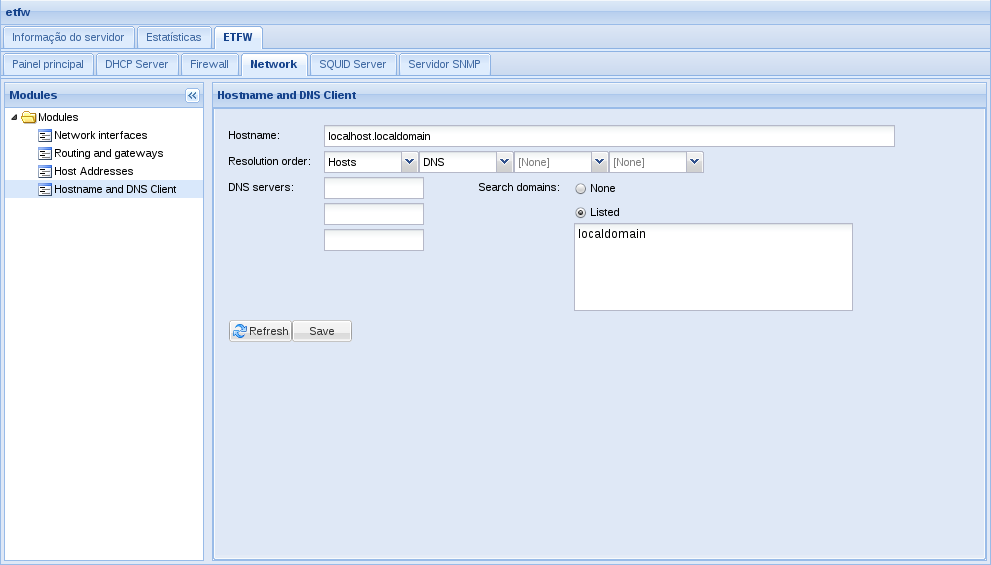
\includegraphics[scale=0.38]{screenshots/etfw/etfw_network_dnsclient_01.png}
    \caption{Cliente DNS}
    \label{fig:etfw_network_dnsclient_01}
    \end{center}
\end{figure}

\subsection{Regras \textit{Firewall}}

Ao aceder ao separador \textit{Firewall} temos a possibilidade de configurar as regras de \textit{Firewall}.
Esta \textit{firewall} é baseada em \textit{iptables}, sendo formada por três ''obectos'' básicos:

\begin{itemize}
    \item Regras
    \item \textit{Chains} (Cadeias)
    \item Tabelas
\end{itemize}

As \textbf{regras} são objectos de nível mais baixo que efectuam a filtragem ou manipulação de pacotes.
Um regra é composta pelas seguintes partes:

\begin{itemize}
\item A tabela a que a regra será adicionada;
\item A \textit{chain} a que a regra será adicionada;
\item As intruções de filtragem ou manipulação.
\end{itemize}

As regras organizam-se em \textbf{chains} e comportam-se como uma lista de verificação de regras ordenadas.

Por sua vez as \textit{chains} organizam-se em \textbf{tabelas} para agrupar a grande quantidade de possibilidades de regras para filtrar e/ou manipular pacotes.

O funcionamento da \textit{firewall} processa-se da seguinte forma: se o cabeçalho do pacote atender aos requisitos da regra, este seguirá o destino imposto pela regra, caso contrário, passará adiante e será avaliado pela próxima regra.
Quando não houver mais regras a avaliar será aplicado ao pacote a regra por omissão ou padrão definida.

\begin{figure}[H]
    \begin{center}
    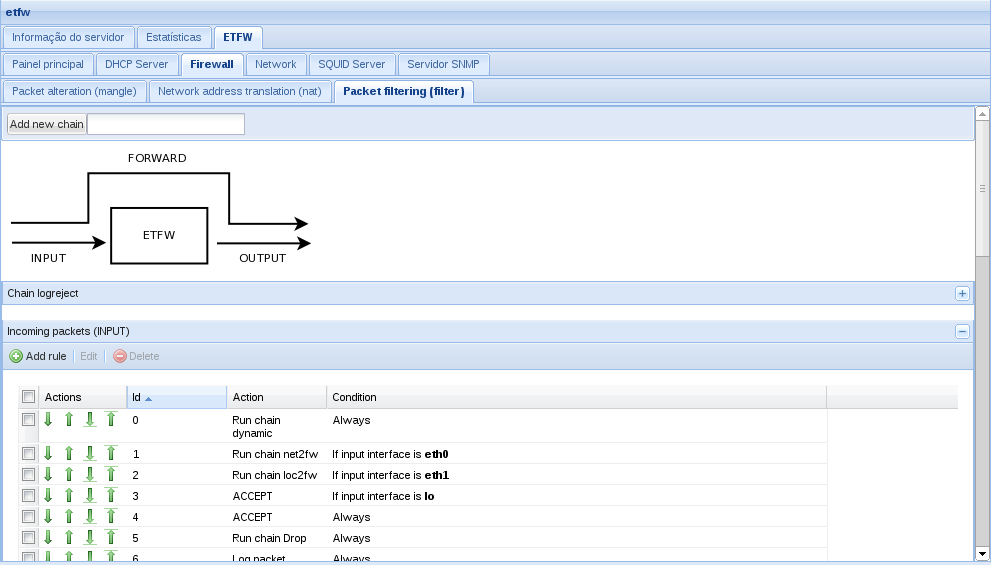
\includegraphics[scale=0.38]{screenshots/etfw/etfw_firewall_01.png}
    \caption{Módulo \textit{Firewall}: Tabela \textit{Filter} }
    \label{fig:etfw_firewall_01}
    \end{center}
\end{figure}

Ao aceder à interface \textit{Firewall} são apresentados os separadores das três tabelas: \textit{Packet alterarion} - \textit{mangle}, \textit{Network address translation} - \textit{nat} e \textit{Packet filtering} - \textit{filter}.

\subsubsection{Tabela \textit{Filter} - \textit{Packet Filtering}}

A tabela \textit{filter} é usada para filtrar pacotes que passem através da \textit{firewall} e apresenta três \textit{chains} pré-definidas:

\begin{itemize}
    \item \textbf{INPUT} - filtra pacotes cujo destino é a própria \textit{firewall};
    \item \textbf{OUTPUT} - filtra pacotes cuja origem é \textit{firewall};
    \item \textbf{FORWARD} - filtra pacotes que passam pela \textit{firewall}, ou sejam, nem são a origem, nem o destino da firewall.
\end{itemize}

\begin{figure}[H]
    \begin{center}
    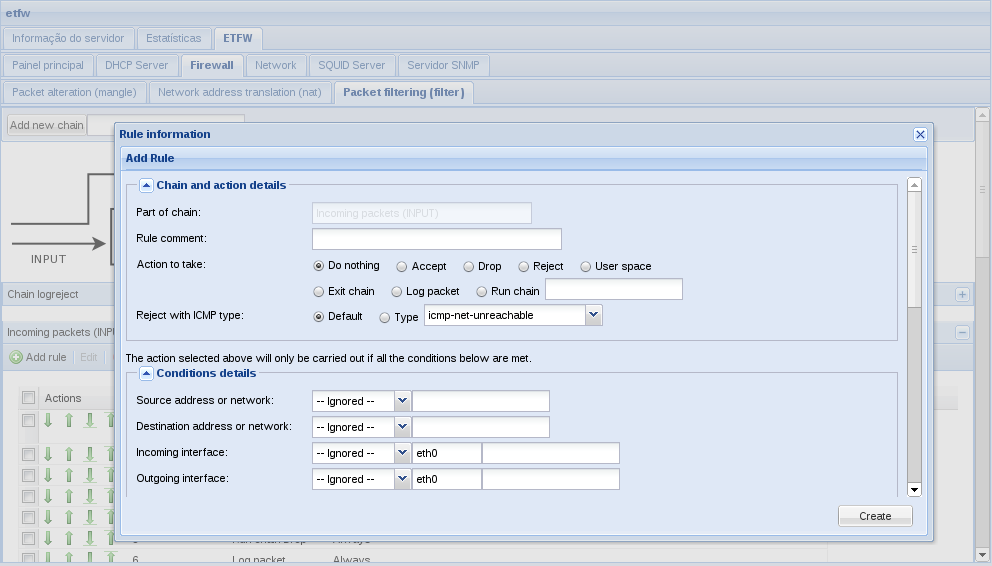
\includegraphics[scale=0.38]{screenshots/etfw/etfw_firewall_02.png}
    \caption{Criar regra na tabela \textit{filter} - \textit{Chain} e acção}
    \label{fig:etfw_firewall_02}
    \end{center}
\end{figure}

Ao criar uma regra numa \textit{chain} da tabela \textit{filter} são solicitados alguns parâmetros para acção a tomar:

\begin{itemize}
    \item \textbf{Rule comment} - permite escrever um pequeno comentário para identificar a regra a ser criada;
    \item \textbf{Action to take} - acção a ser tomada, que decide o que deverá ser feito com o pacote se este corresponder à regra. As acções mais importantes são:
        \subitem \textbf{Drop} - elimina o pacote sem fazer mais nada;
        \subitem \textbf{Accept} - a \textit{firewall} deixa o pacote passar e os dados são enviados para o destinatário;
        \subitem \textbf{Reject} - funciona da mesma forma que o \textbf{Drop} mas é enviado um erro \textit{ICMP} de volta ao emissor do pacote;
        \subitem \textbf{Userspace} - se esta opção estiver activa é feito, pelo \textit{kernel}, o \textit{multicast} do pacote para um \textit{socket} na qual pode estar à escuta um processo.
\end{itemize}

\begin{figure}[H]
    \begin{center}
    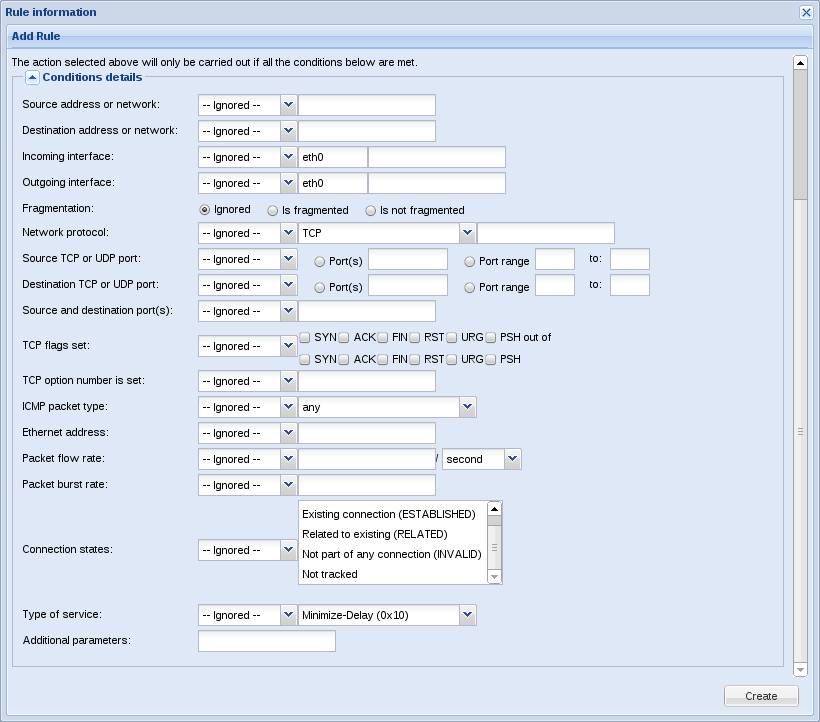
\includegraphics[scale=0.38]{screenshots/etfw/etfw_firewall_03.png}
    \caption{Criar regra na tabela \textit{filter} - Detalhes da condição}
    \label{fig:etfw_firewall_03}
    \end{center}
\end{figure}

Outras opções que podem ser completadas na condição são as seguintes:

\begin{itemize}
    \item \textbf{Source address or network} - Endereço ou rede que estabelece a origem do pacote. Geralmente é uma combinação do endereço IP com a máscara de subrede separadas por barra (Ex: 192.168.1.0/255.255.255.0 ou 192.168.1.0/24);
    \item \textbf{Destination address or network} - Endereço ou rede a que se destina o pacote. Tem a mesma combinação que o anterior;
    \item \textbf{Incoming interface} - Especifica a interface de entrada do pacote;
    \item \textbf{Outgoing interface} - Especifica a interface de saída do pacote;
    \item \textbf{Fragmentation} - Algumas vezes um pacote sofre fragmentação devido ao seu tamanho, sendo rescontruído, posteriormente, no destino. Esta opção permite definir se a regra faz correspondência através de pacotes fragmentados ou não;
    \item \textbf{Network protocol} - Correspondência ao protocolo de rede;
    \item \textbf{Source TCP or UDP port} - Define a correspondência por porta de entrada (\textit{TCP} ou \textit{UDP}), podendo ser facultado um intervalo de portas (exemplo: 1000:1050) ou uma lista de portas separadas por vírgulas;
    \item \textbf{Destination TCP or UDP port} - Define a correspondência por porta de saída, podendo ser facultado um intervalo de portas (exemplo: 1000:1050) ou uma lista de portas separadas por vírgulas;
    \item \textbf{Source and destination port(s)} - Define a correspondência pela porta, tanto de entrada como de saída, podendo ser facultado um intervalo de portas ou uma lista de portas separadas por vírgulas;
    \item \textbf{ICMP packet type} - Tipo de pacote \textit{ICMP} que vai fazer corespondência;
    \item \textbf{Ethernet address} - Identifica um endereço físico de rede que servirá para fazer correspondência com a regra;
    \item \textbf{Packet flow rate} - Define o volume de pacotes com que a regra passará a fazer correspondência;
    \item \textbf{Packet burst rate} - Define o limite a partir do qual os pacotes começarão a fazer correspondência com a regra;
    \item \textbf{Connection states} - Específica o conjunto de estados da ligação que fazem correspondência;
    \item \textbf{Type of service} - Define o tipo de serviço para o qual desejamos que a regra faça correspondência;
    \item \textbf{Additional parameters} - Especifica parâmetros adicionais que vão ser passados directamente para a linha da regra da \textit{firewall} a ser executada.
\end{itemize}

\subsubsection{Tabela \textit{NAT} - \textit{Network address translation}}

A tabela \textit{NAT} é usada para tradução do endereço de rede (\textit{Network Address Translation}), ou seja, traduzir uma pacote com um determinado campo de origem ou destino.
Apenas o primeiro pacote será atingido por esta \textit{chain}, após isto, os restantes pacotes, serão aplicadas as mesmas acções do primeiro.
Esta tabela apresenta três \textit{chains} pré-definidas:

\begin{itemize}
    \item \textbf{PREROUTING} - aplica as alterações aos pacotes quando o destino necessita de ser alterado;
    \item \textbf{POSTROUTING} - aplica as alterações aos pacotes quando a origem necessita de ser alterada;
    \item \textbf{OUTPUT} - aplic as alterações aos pacotes originados pela \textit{firewall}.
\end{itemize}

Os alvos actuais desta tabela são:

\begin{itemize}
    \item \textbf{DNAT} - usado nos casos em que se tem um endereço IP público na \textit{firewall} e se quer redireccionar o acesso para outro \textit{host} (numa \textit{DMZ} por exemplo), permitindo assim encaminhar o tráfego.
    \item \textbf{SNAT} - usado quando se quer alterar a origem do pactoe, normalmente para esconder os endereços locais da rede ou \textit{DMZ}.
    \item \textbf{MASQUERADE} - usado da mesma forma que o \textit{SNAT} e para o mesmo motivo, mas o endereço IP de saída não é especificado, sendo utilizado o endereço de origem da interface de saída do pacote. Esta regra é usada principalmente para endereços IPs dinâmicos, pois se a ligação for abaixo, o endereço de origem que estava a ser utilizado é descartado, dando lugar ao novo endereço de origem da interface quando a ligação for restabelecida.
\end{itemize}

\begin{figure}[H]
    \begin{center}
    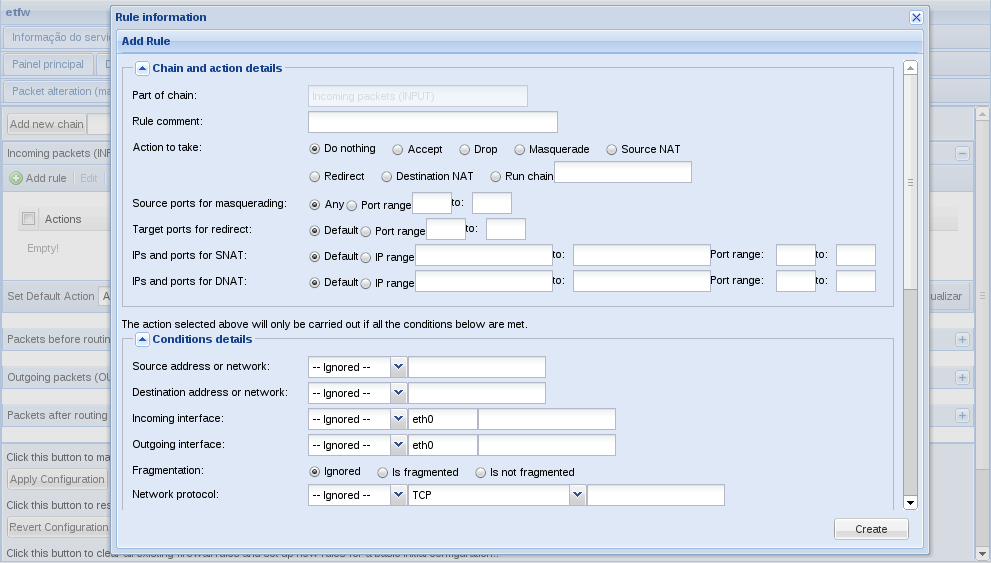
\includegraphics[scale=0.38]{screenshots/etfw/etfw_firewall_04.png}
    \caption{Criar regra na tabela \textit{NAT}}
    \label{fig:etfw_firewall_03}
    \end{center}
\end{figure}

As opções utilizadas na tabela \textit{NAT} são idênticas às da tabela \textit{filter}, diferenciado nas seguintes opções:

\begin{itemize}
    \item \textbf{Action to take} - acção a ser tomada, tem a mesma funcionalidade descrita na tabela \textit{filter}, mas possui duas opções diferentes:
        \subitem \textbf{Masquerade} - Re-escreve o endereço IP de saída, quando se trata de endereços IPs dinâmicos;
        \subitem \textbf{Source NAT} / \textbf{Destination NAT} - Dependendo da \textit{chain} (\textit{PREROUTING}, \textit{POSTROUTING} ou \textit{OUTPUT}) a opção disponível pode variar entre \textbf{Source NAT} e \textbf{Destination NAT}. Re-escrevem os endereços IP's de entrada e saída respectivamente.
\end{itemize}

\subsubsection{Tabela \textit{Mangle} - \textit{Packet alteration}}

Esta tabela não será abordada nesta versão do manual.

\subsection{Servidor \textit{DHCP}}

Neste separador podemos configurar o servidor de DHCP, nomeadamente, intervalo de IPs a alocar a \textit{hosts}, endereço de encaminhador, endereço de servidor DNS, visualizar concessões activas, e até iniciar/parar o servidor.

\begin{figure}[H]
    \begin{center}
    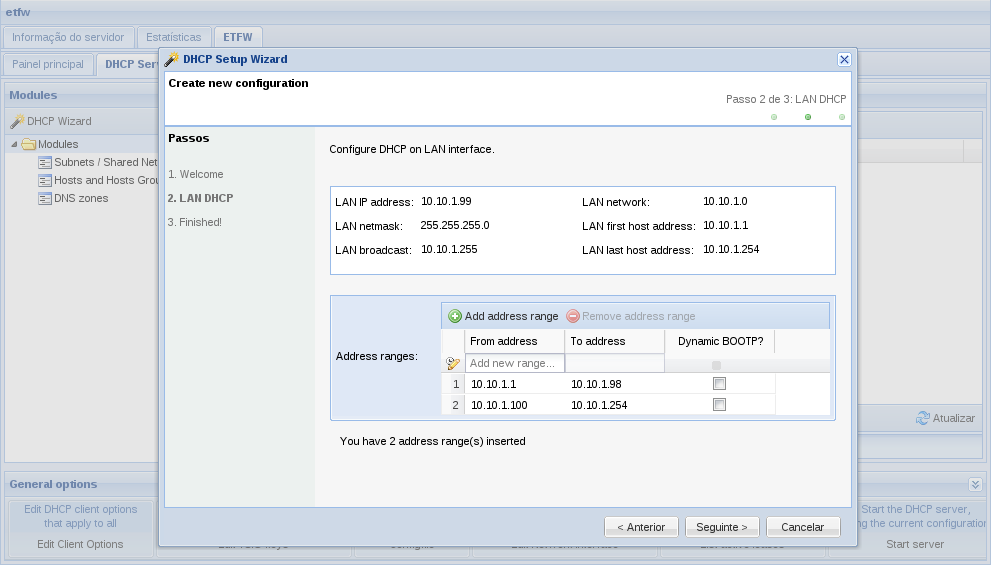
\includegraphics[scale=0.38]{screenshots/etfw/etfw_dhcp_wizard_01.png}
    \caption{Configuração dos intervalos de IP}
    \label{fig:etfw_dhcp_wizard_01}
    \end{center}
\end{figure}

A partir do \textit{DHCP Wizard} podemos, numa primeira fase, configurar os intervalos de IP alocados para \textit{hosts}.

\begin{figure}[H]
    \begin{center}
    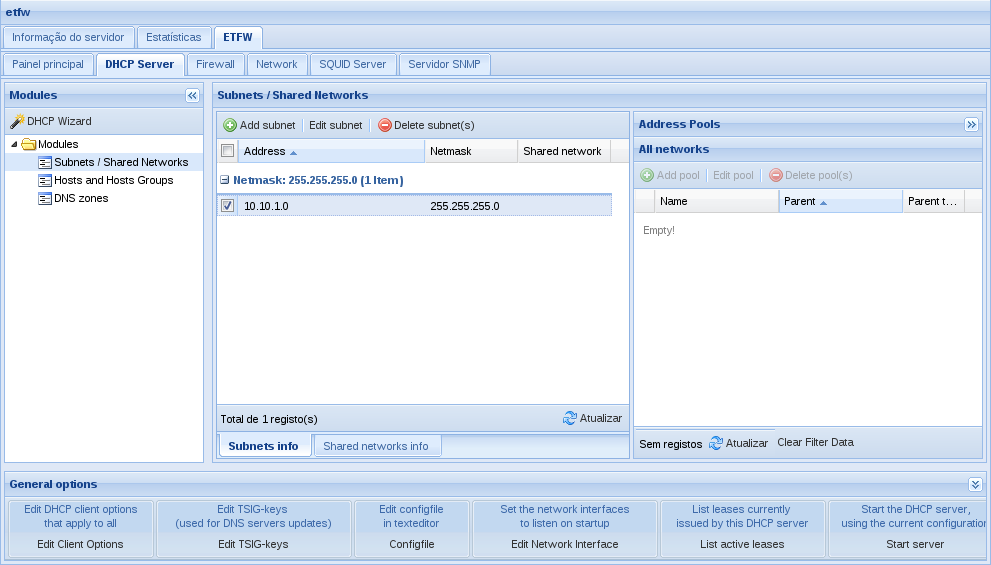
\includegraphics[scale=0.38]{screenshots/etfw/etfw_dhcp_subnets_01.png}
    \caption{Configuração sub-redes}
    \label{fig:etfw_dhcp_subnets_01}
    \end{center}
\end{figure}

\begin{figure}[H]
    \begin{center}
    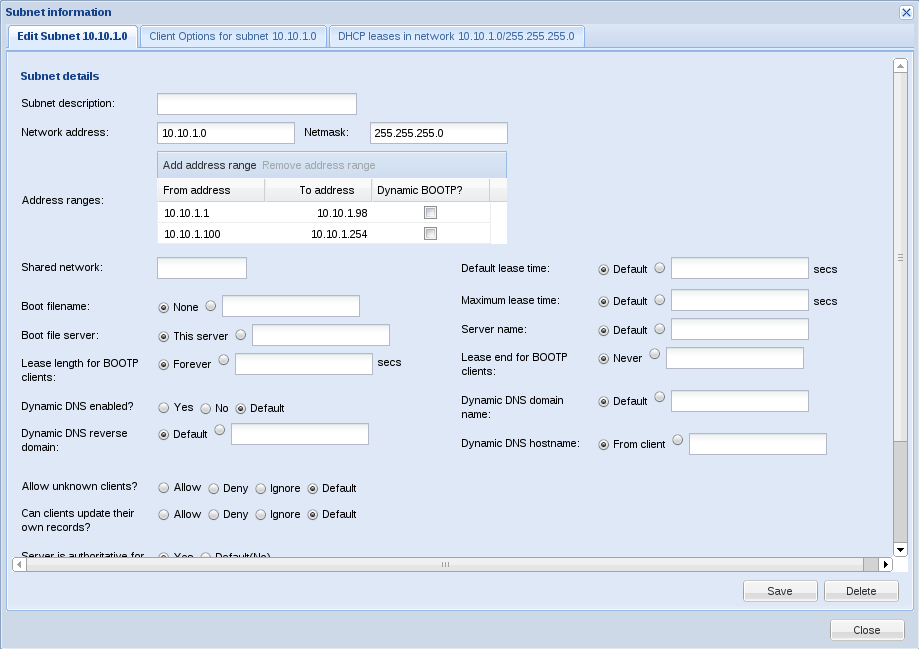
\includegraphics[scale=0.38]{screenshots/etfw/etfw_dhcp_subnets_02.png}
    \caption{Editar sub-rede}
    \label{fig:etfw_dhcp_subnets_02}
    \end{center}
\end{figure}

Posteriormente, é possível editar as sub-redes e definir os parâmetros adequados à nossa configuração para endereço de rede (\textit{Network address}) , máscara de rede (\textit{netmask}), intervalo de endereços (\textit{Address ranges}), entre outros.

\begin{figure}[H]
    \begin{center}
    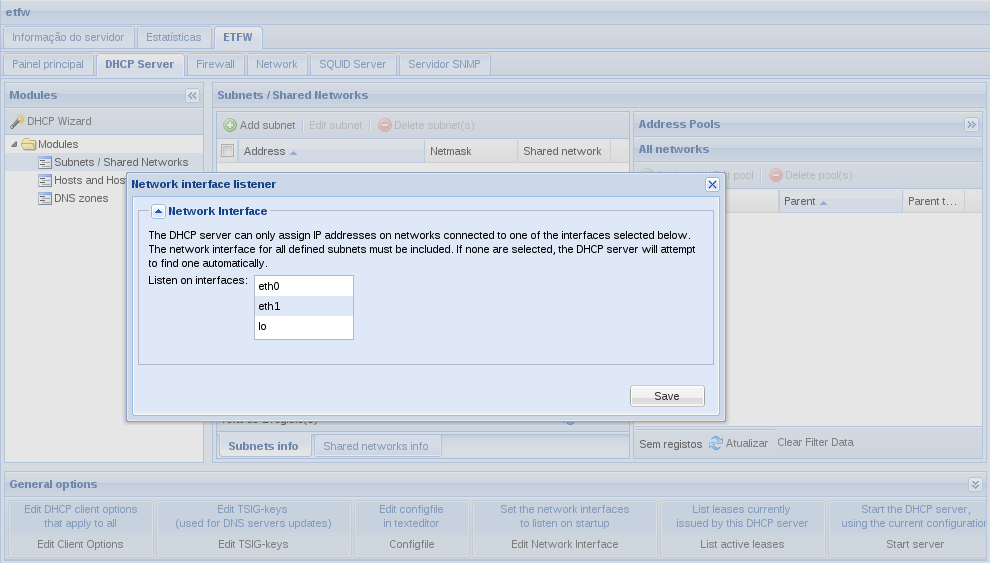
\includegraphics[scale=0.38]{screenshots/etfw/etfw_dhcp_interfaces_01.png}
    \caption{Escolha de interface}
    \label{fig:etfw_dhcp_interfaces_01}
    \end{center}
\end{figure}

Para configurar o servidor devidamente é necessário definir a interface em que serviço vai operar.
Para isso escolhemos a opção \textit{Edit Network Interface} e escolhemos a interface de rede pretendida.

\begin{figure}[H]
    \begin{center}
    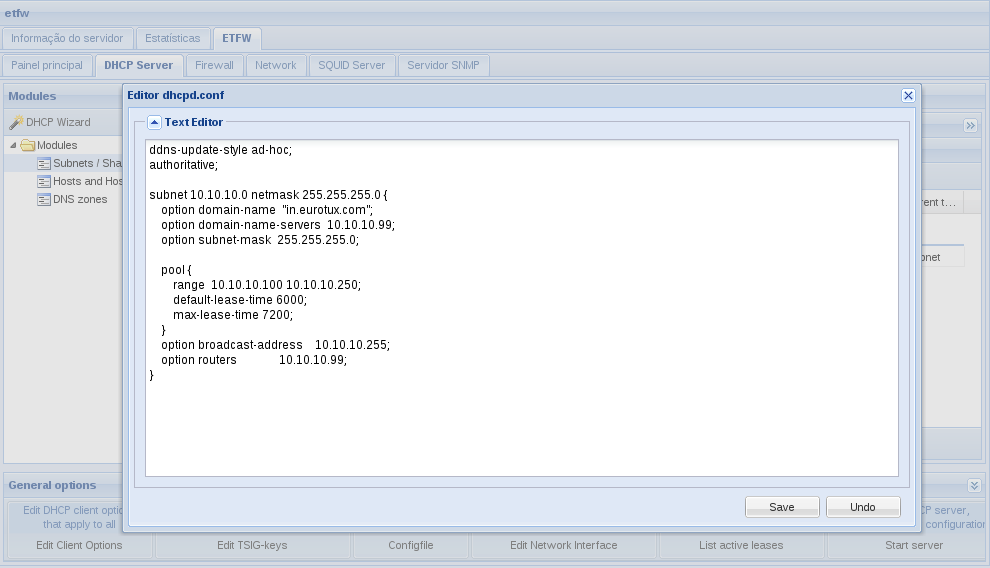
\includegraphics[scale=0.38]{screenshots/etfw/etfw_dhcp_texteditor_01.png}
    \caption{Edição do ficheiro de configuração}
    \label{fig:etfw_dhcp_texteditor_01}
    \end{center}
\end{figure}

Adicionalmente, é sempre possível visualizar e editar o ficheiro de configuração directamente e colocar as opções pretendidas.

\begin{figure}[H]
    \begin{center}
    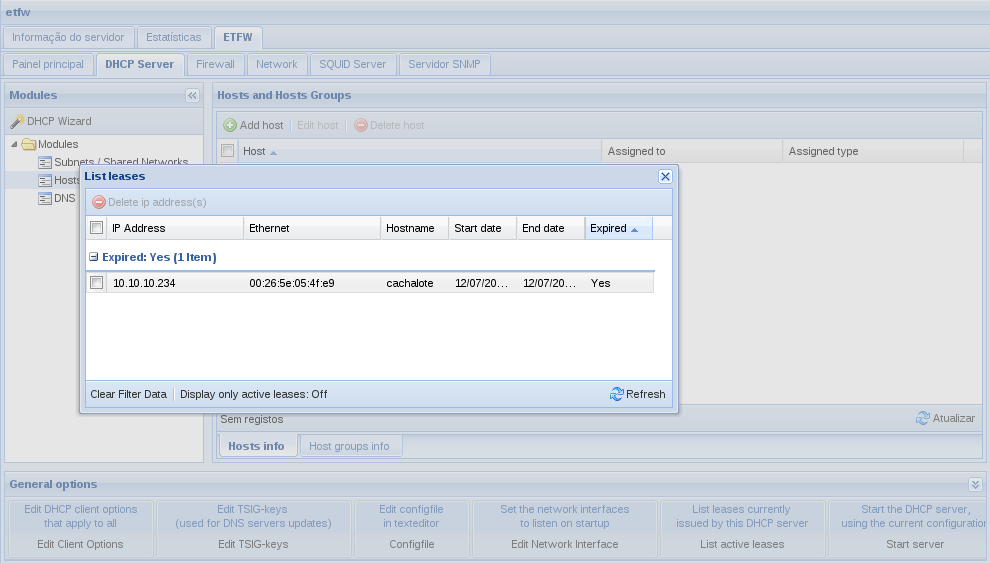
\includegraphics[scale=0.38]{screenshots/etfw/etfw_dhcp_leases_01.png}
    \caption{Lista de concessões activas}
    \label{fig:etfw_dhcp_leases_01}
    \end{center}
\end{figure}

A qualquer altura é possível consultar a lista de IPs atribuídos através da opção \textit{List active leases}. Esta opção também se encontra disponível para cada sub-rede.

\subsection{Servidor \textit{SQUID}}

No separador \textit{Servidor SQUID} é possível configurar o serviço de \textit{Proxy} \textit{SQUID}.

\begin{figure}[H]
    \begin{center}
    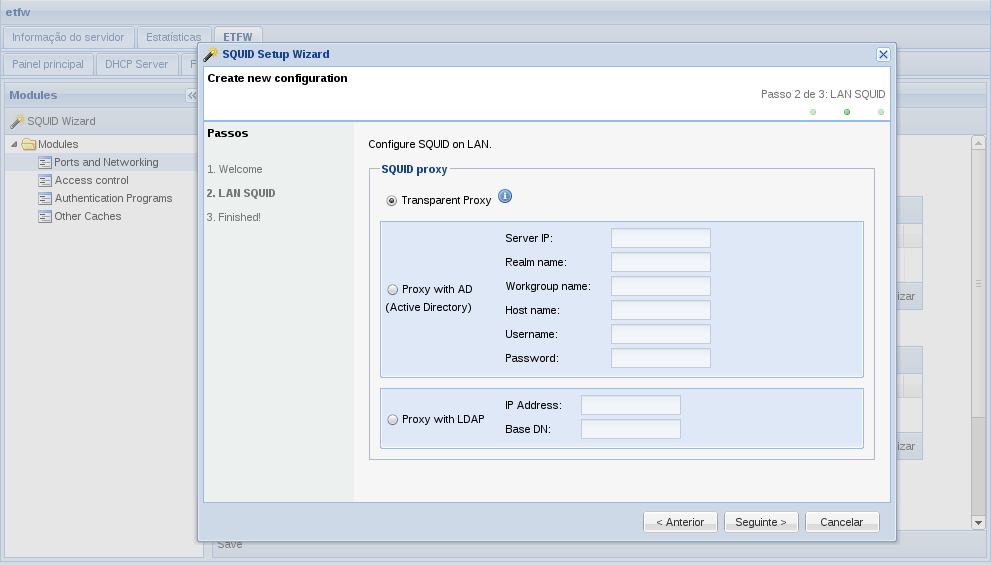
\includegraphics[scale=0.38]{screenshots/etfw/etfw_squid_wizard_01.png}
    \caption{Configuração do servidor SQUID}
    \label{fig:etfw_squid_wizard_01}
    \end{center}
\end{figure}

O serviço de \textit{proxy} tem a função de encaminhar os pedidos para a Internet e guardar uma \textit{cache} dos conteúdos de forma a acelerar a visualização quando forem solicitados novamente.

Na opção \textit{SQUID Wizard} podemos configurar o serviço de \textit{proxy} de forma imediata, tendo ao dispôr três opções configuração pré-definidas:

\begin{itemize}
    \item \textit{Transparent Proxy} - \textit{Proxy} transparente;
    \item \textit{Proxy with AD} - \textit{Proxy} com autenticação em \textit{Active Directory};
    \item \textit{Proxy with LDAP} - \textit{Proxy} com autenticação em \textit{LDAP}.
\end{itemize}

No primeiro caso, o \textit{Proxy} transparente, permite ter um sistema de \textit{cache} totalmente invisível aos \textit{browsers} dos clientes. Este sistema não suporta autenticação.

Nos outros dois casos, o \textit{Proxy} faz uso de sistemas de autenticação, como \textit{Active Directory} ou \textit{LDAP}.

Adicionalmente, é possível configurar de forma avançada o serviço \textit{Proxy} de acordo com as necessidades, nomeadamente, \textit{Ports and Networking}, \textit{Access Control}, \textit{Authentication Programs} e \textit{Other Caches}.

\subsubsection{\textit{Ports and Networking}}

Em \textit{Ports and Networking} é possível definir as portas ( \textit{SSL} ou não ) e endereços IP ou nome da máquina onde o serviço \textit{proxy} vai atender pedidos, para além de outras configurações possíveis, nomeadamente:

\begin{figure}[H]
    \begin{center}
    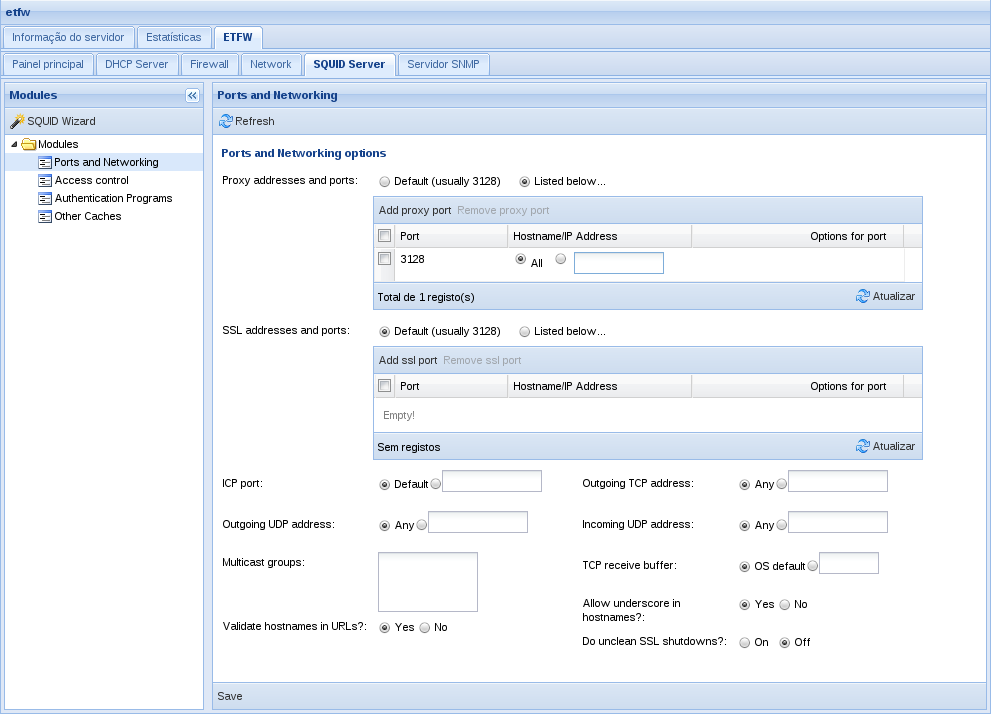
\includegraphics[scale=0.38]{screenshots/etfw/etfw_squid_portsnetworking_01.png}
    \caption{Configuração de portas e rede}
    \label{fig:etfw_squid_portsnetworking_01}
    \end{center}
\end{figure}

\begin{itemize}
    \item \textit{ICP port} - Porta de pedidos \textit{ICP};
    \item \textit{Validate hostnames in URLs?} - Validação nome de endereços dos \textit{URLs};
    \item \textit{Multicast groups} - Especificação de grupos \textit{multicast};
    \item \textit{Outgoing TCP address} - Endereço de saída de tráfego TCP;
    \item \textit{Outgoing UDP address} - Endereço de saída de tráfego UDP;
    \item \textit{Incoming UDP address} - Endereço de entrada de tráfego UDP;
    \item \textit{TCP receive buffer} - Parametrização de buffer \textit{TCP};
\end{itemize}

\subsubsection{\textit{Access Control}}

Em \textit{Access Control} definimos as políticas de controlo de acessos baseadas na combinação de \textit{ACLs} (\textit{Access Control lists}).

\begin{figure}[H]
    \begin{center}
    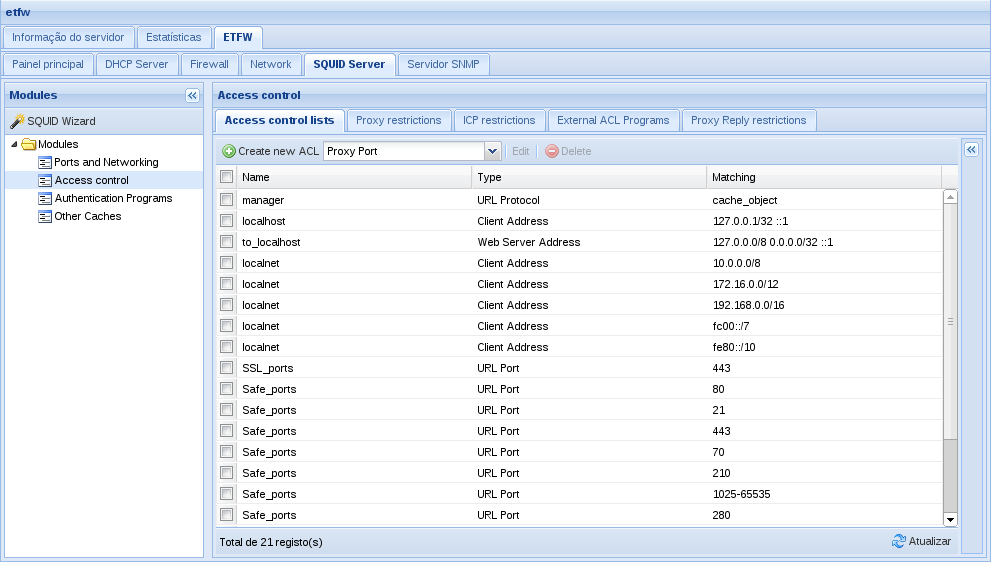
\includegraphics[scale=0.38]{screenshots/etfw/etfw_squid_accesscontrol_01.png}
    \caption{Configuração de políticas de controlo de acesso - \textit{ACLs}}
    \label{fig:etfw_squid_accesscontrol_01}
    \end{center}
\end{figure}

Na configuração de políticas de controlo de acesso podemos definir os modelos de filtragem passíveis de serem utilizadas, posteriormente, nas secções de restrições de accesso (\textit{Proxy restrictions}, \textit{ICP restrictions}, \textit{Proxy Reply restrictions}).

\begin{figure}[H]
    \begin{center}
    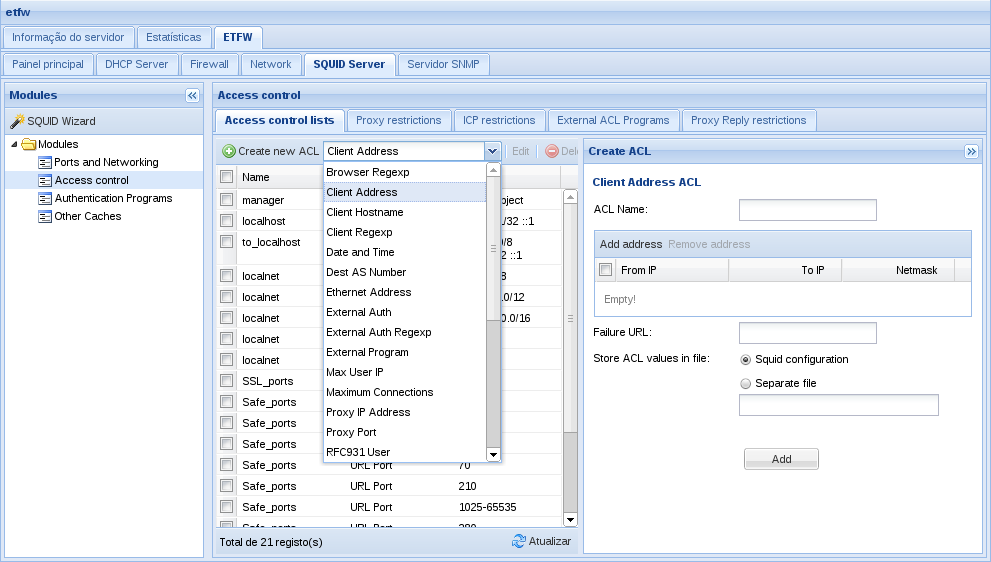
\includegraphics[scale=0.38]{screenshots/etfw/etfw_squid_accesscontrol_02.png}
    \caption{Criar nova \textit{ACLs}}
    \label{fig:etfw_squid_accesscontrol_02}
    \end{center}
\end{figure}

Para criar uma nova \textit{ACL}, específicamos o tipo e preenchemos com os parâmetros pretendidos.

\begin{figure}[H]
    \begin{center}
    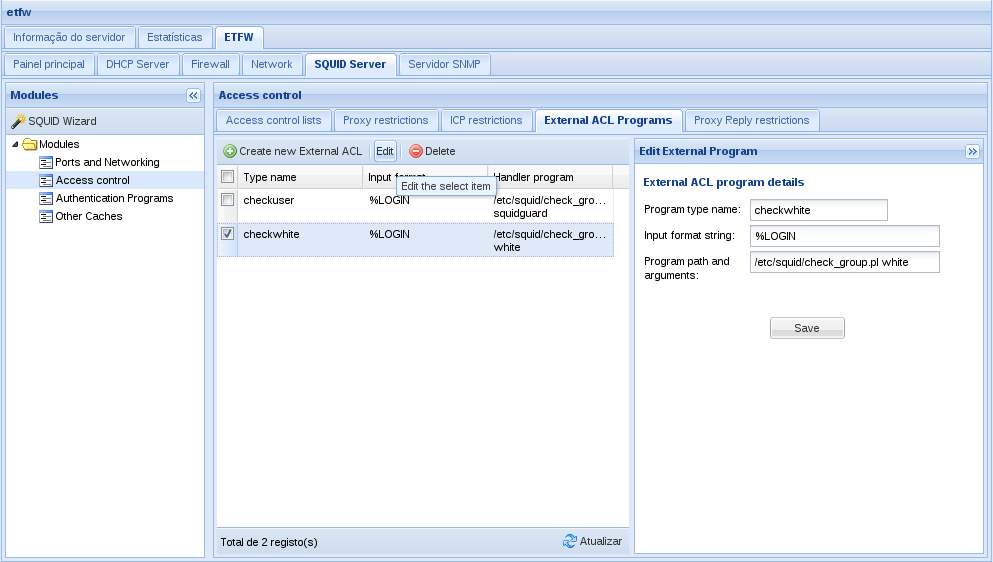
\includegraphics[scale=0.38]{screenshots/etfw/etfw_squid_accesscontrol_03.png}
    \caption{Criar nova \textit{External ACLs}}
    \label{fig:etfw_squid_accesscontrol_03}
    \end{center}
\end{figure}

É também possível definir \textit{ACLs} externas que permitem expandir as funcionalidades do \textit{proxy} utilizando para isso programs externos para gerir os acessos.
Estas \textit{ACLs} possibilitam, por exemplo, a autenticação num servidor \textit{Active Directory} ou \textit{LDAP}, ou ainda, a verificação de endereços de origem numa base de dados \textit{SQL}.

A criação de um \textit{ACL} externa perssupõe a criação de uma \textit{ACL} interna com referência à primeira.

\begin{figure}[H]
    \begin{center}
    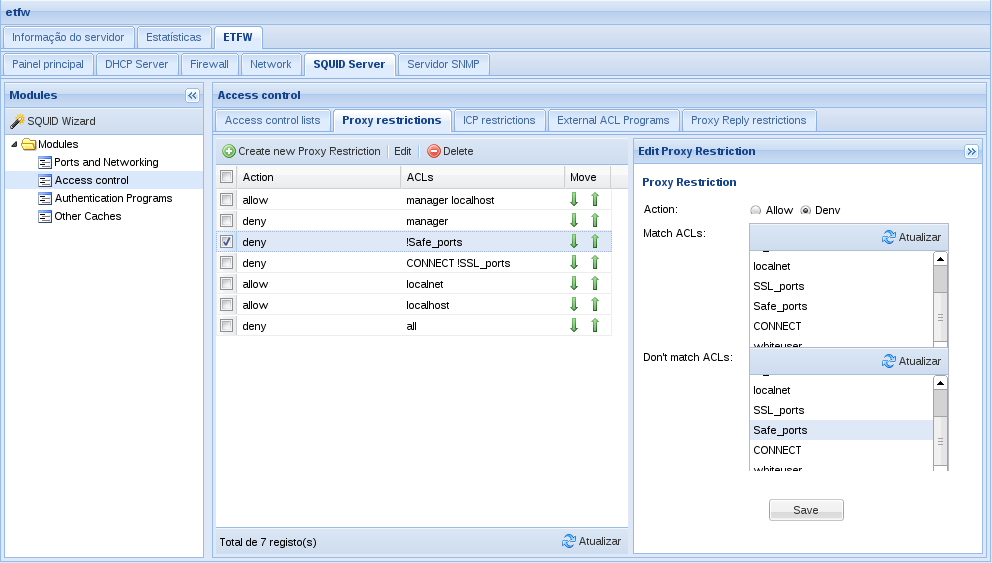
\includegraphics[scale=0.38]{screenshots/etfw/etfw_squid_accesscontrol_04.png}
    \caption{Definição de uma restrição - \textit{Proxy restrictions}}
    \label{fig:etfw_squid_accesscontrol_04}
    \end{center}
\end{figure}

Após a definição das \textit{ACLs}, é necessário definir as restrições com as combinações das \textit{ACLs} a aplicar em cada situação, ou seja, qual a acção a fazer: negar ou aceita.
As regras são aplicadas por ordem, de cima para baixo, e quando é encontrada uma correspondência a acção é efectuada.
É importante salientar que caso não exista uma regra de negação (\textit{deny all}), todos os pedidos que passem as regras são aceites.

\subsubsection{\textit{Authentication Programs}}

Em \textit{Authentication Programs} são definidos os programas de autenticação que perguntam ao \textit{browser}/utilizador quais os seus dados de autenticação.

\begin{figure}[H]
    \begin{center}
    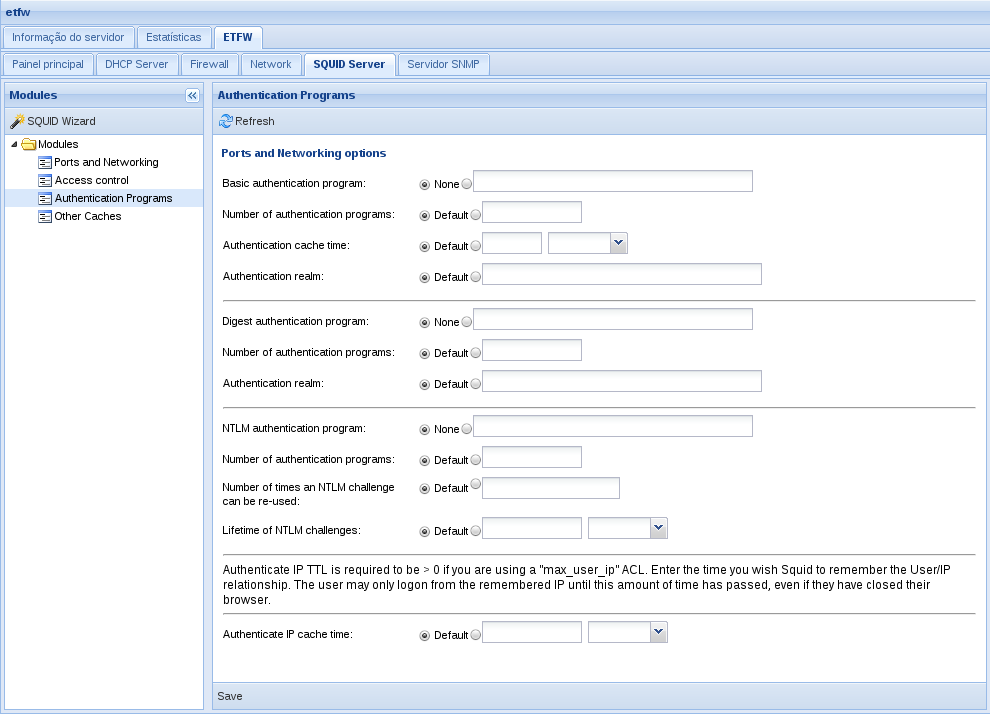
\includegraphics[scale=0.38]{screenshots/etfw/etfw_squid_authenticationprograms_01.png}
    \caption{Programas de autenticação - \textit{Authentication Programs}}
    \label{fig:etfw_squid_authenticationprograms_01}
    \end{center}
\end{figure}

Existem dois modelos de autenticação:

\begin{itemize}
    \item \textit{Basic} - quando o \textit{browser} não suporta aunteticação transparente aparece um \textit{popup} para introdução de dados de autenticação
    \item \textit{NTLMSSP} - autenticação transparente para o utilizador
\end{itemize}

E podem receber os seguintes parâmetros:

\begin{itemize}
    \item \textit{authentication program} - Especifica o programa utilizador para autenticação. O programa lê uma linha contendo utilizador e \textit{password} separado por espaço e responde \textit{OK} em caso de sucesso ou \textit{ERR} em caso de falha;
    \item \textit{Number of authentication programs} - Número de processo que o pgroama de autenticação poderá conter;
    \item \textit{Authentication realm} - Texto que irá ser apresentado na caixa de diálogo para o caso de autenticação \textit{basic};
    \item \textit{Authentication cache time} - Especifica por quanto tempo uma autenticação válida é mantida sem nova solicitação;
    \item \textit{Number of times an NTLM challenge can be re-used} - Número máximo que uma autenticação pode ser usada para o tipo de autenticação \textit{NTLMSSP};
    \item \textit{Lifetime of NTLM challenges} - Tempo de vida de autenticação do tipo \textit{NTLMSSP};
    \item \textit{Authenticate IP cache time} - Especifica por quanto tempo é mantida em \textit{cache} a relação de um utilização a determinado \textit{IP}.
\end{itemize}

\subsubsection{\textit{Other Caches}}

Em \textit{Other Caches} é possível especificar outras \textit{proxies} que serão usados em cadeia para obter informação.

\begin{figure}[H]
    \begin{center}
    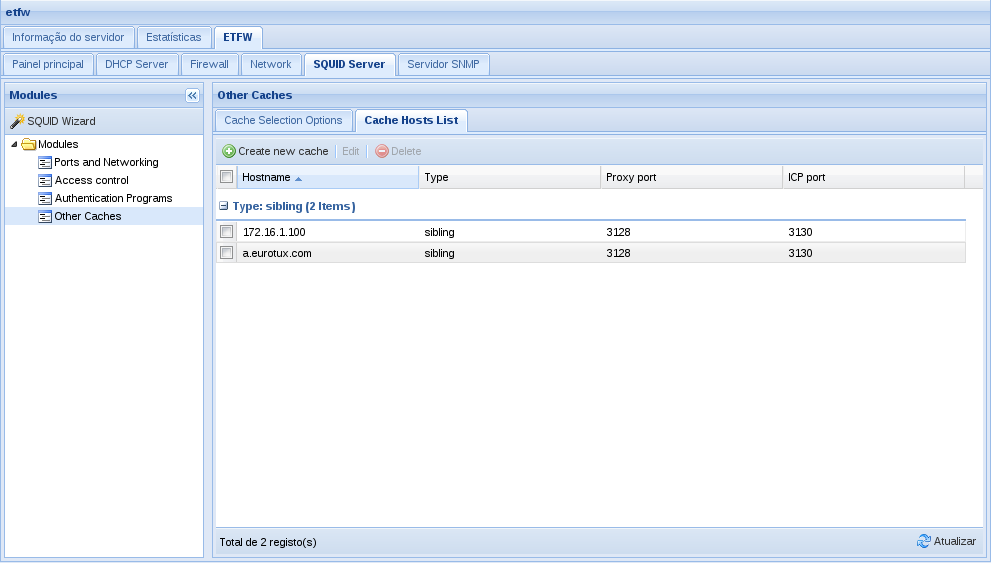
\includegraphics[scale=0.38]{screenshots/etfw/etfw_squid_othercaches_01.png}
    \caption{\textit{Proxies} - \textit{Other Caches}}
    \label{fig:etfw_squid_othercaches_01}
    \end{center}
\end{figure}

\begin{figure}[H]
    \begin{center}
    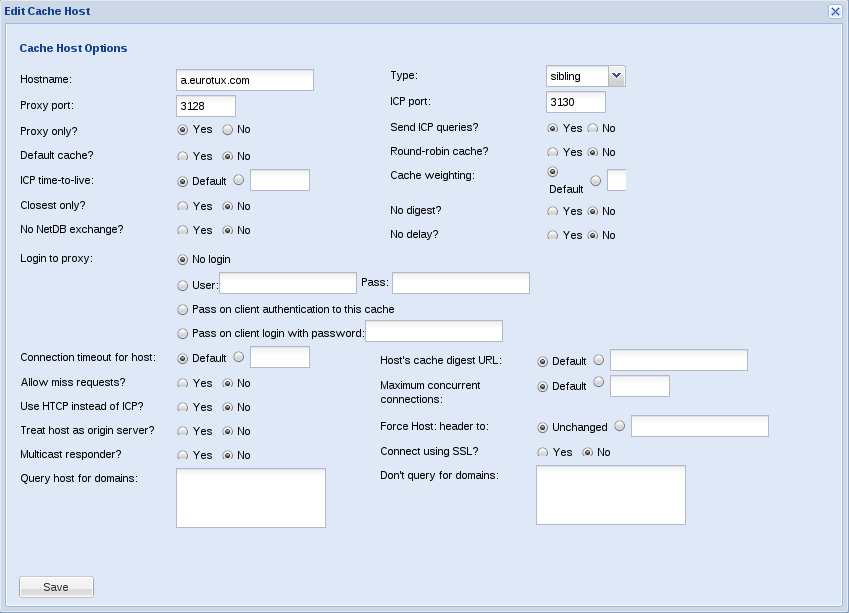
\includegraphics[scale=0.38]{screenshots/etfw/etfw_squid_othercaches_02.png}
    \caption{Editar \textit{Cache} \textit{Host}}
    \label{fig:etfw_squid_othercaches_01}
    \end{center}
\end{figure}

Para especificar outro \textit{proxy} é necessário especificar os seguintes campos:

\begin{itemize}
    \item \textit{Hostname} - Endereço IP ou \textit{hostname} (\textit{FQDN}) da cache a ser utilizada;
    \item \textit{Type} - Tipo de hierarquia a utilizar entre os \textit{proxies}:
        \subitem \textit{parent};
        \subitem \textit{sibling};
        \subitem \textit{multicast};
    \item \textit{Proxy port} - A porta onde o \textit{proxy} está à espera dos pedidos;
    \item \textit{ICP port} - A porta usada para perguntar aos vizinhos sobre os objectos que as caches possam ter ou não;
    \item \textit{Proxy only?} - Indica que o conteúdo pedido a este \textit{proxy} não é para guardar localmente;
    \item \textit{Send ICP queries} - Usado para \textit{proxies} que não usam \textit{ICP}, ou seja, que não indicam se contêm um objecto ou não;
    \item \textit{Default cache} - Usa-se quando o \textit{proxy} é o último na linha hierárquica;
    \item \textit{Round-robin cache} - Para usar algoritmo \textit{round-robin} de consulta de \textit{proxies} ;
    \item \textit{ICP time-to-live} - Especifica o \textit{Time-To-Live} (\textit{ttl}) usado em \textit{multicast};
    \item \textit{Cache weighting} - Especifica o peso na escolha do \textit{proxy} (por omissão é 1 e quanto maior for mais ''favorecido'' será este \textit{proxy}).
\end{itemize}

\subsubsection{Exemplos de utilização}

\begin{figure}[H]
    \begin{center}
    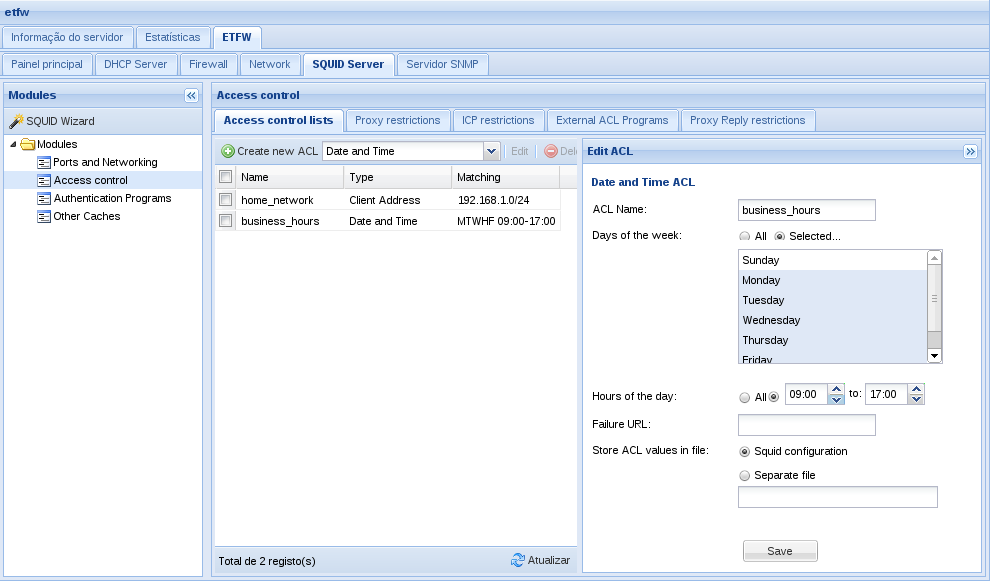
\includegraphics[scale=0.38]{screenshots/etfw/etfw_squid_example_time_01_01.png}
    \caption{Restringir acessos da rede interna apenas em horário de trabalho - Criar \textit{ACLs}}
    \label{fig:etfw_squid_example_time_01_01}
    \end{center}
\end{figure}

\begin{figure}[H]
    \begin{center}
    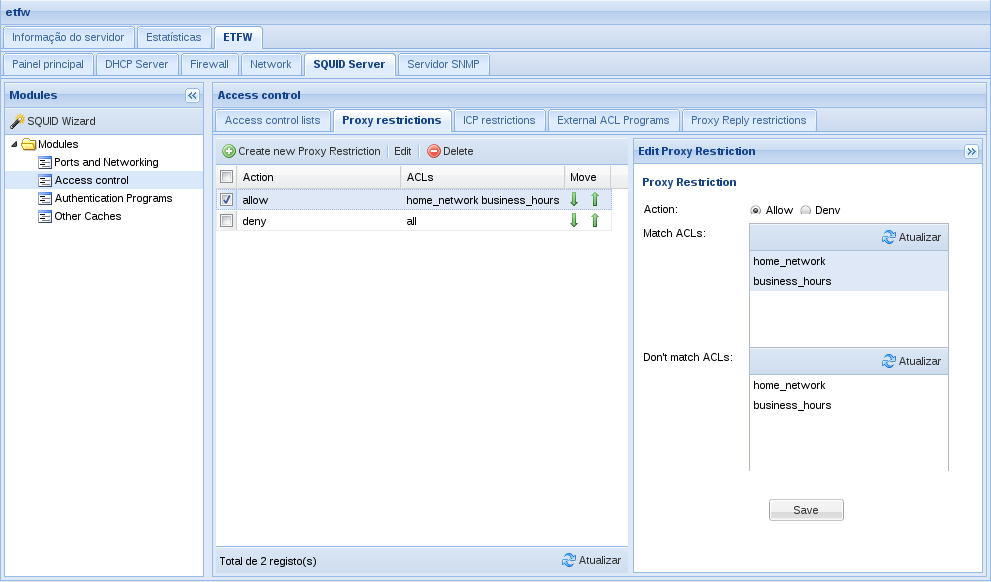
\includegraphics[scale=0.38]{screenshots/etfw/etfw_squid_example_time_01_02.png}
    \caption{Restringir acessos da rede interna apenas em horário de trabalho - Criar restrição usando as \textit{ACLs} anteriores}
    \label{fig:etfw_squid_example_time_01_02}
    \end{center}
\end{figure}

\begin{figure}[H]
    \begin{center}
    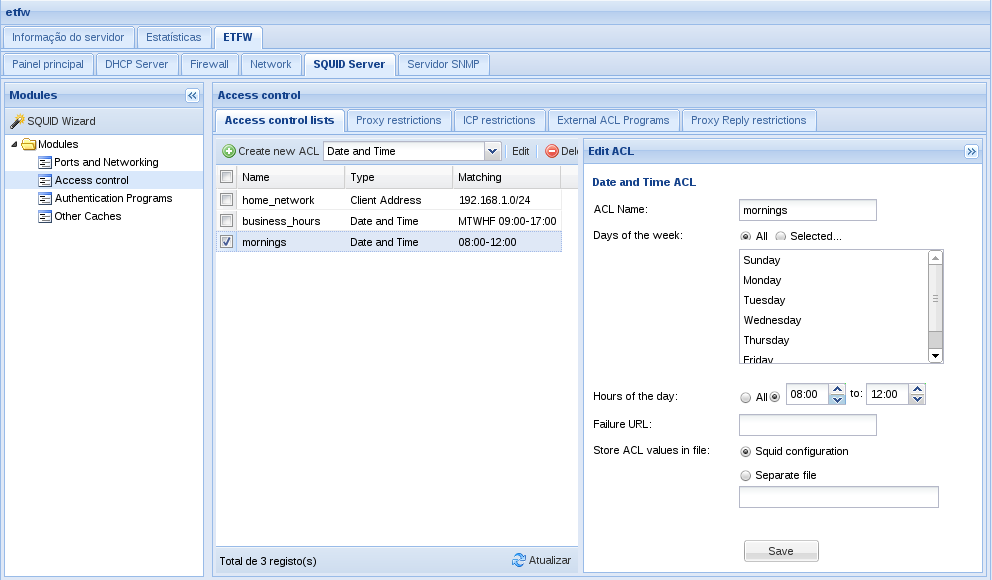
\includegraphics[scale=0.38]{screenshots/etfw/etfw_squid_example_time_02_01.png}
    \caption{Restringir acesso apenas de manhã - Criar \textit{ACLs}}
    \label{fig:etfw_squid_example_time_02_01}
    \end{center}
\end{figure}

\begin{figure}[H]
    \begin{center}
    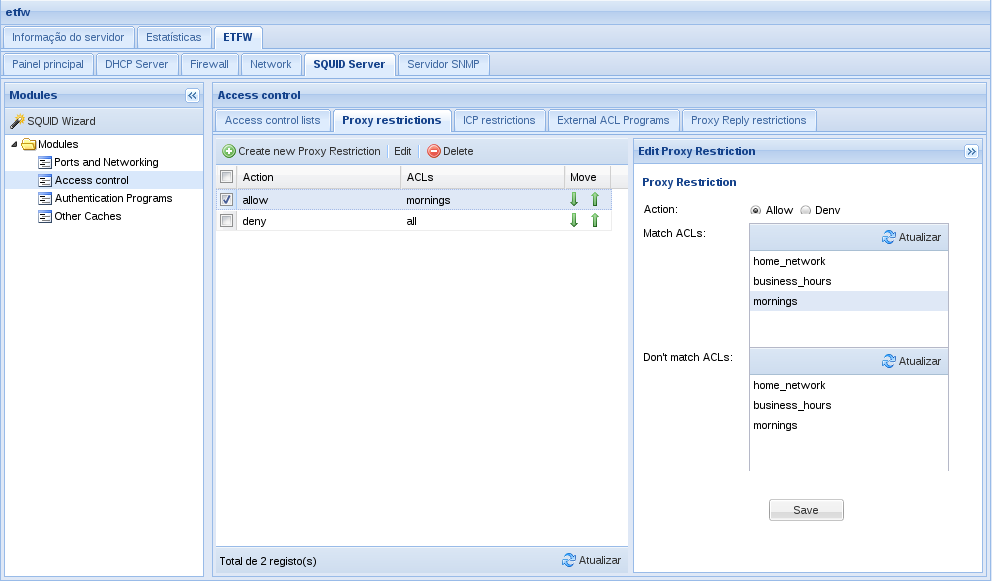
\includegraphics[scale=0.38]{screenshots/etfw/etfw_squid_example_time_02_02.png}
    \caption{Restringir acesso apenas de manhã - Criar restrição usando as \textit{ACLs} anteriores}
    \label{fig:etfw_squid_example_time_02_02}
    \end{center}
\end{figure}

\begin{figure}[H]
    \begin{center}
    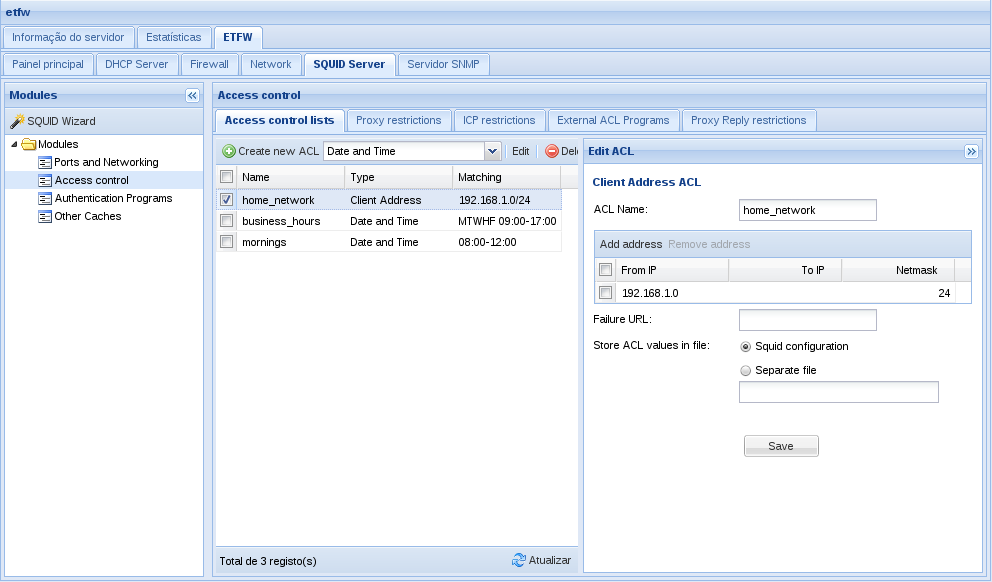
\includegraphics[scale=0.38]{screenshots/etfw/etfw_squid_example_acessoip_01.png}
    \caption{Restringir acessos pelo endereço IP - Criar \textit{ACLs}}
    \label{fig:etfw_squid_example_acessoip_01}
    \end{center}
\end{figure}

\begin{figure}[H]
    \begin{center}
    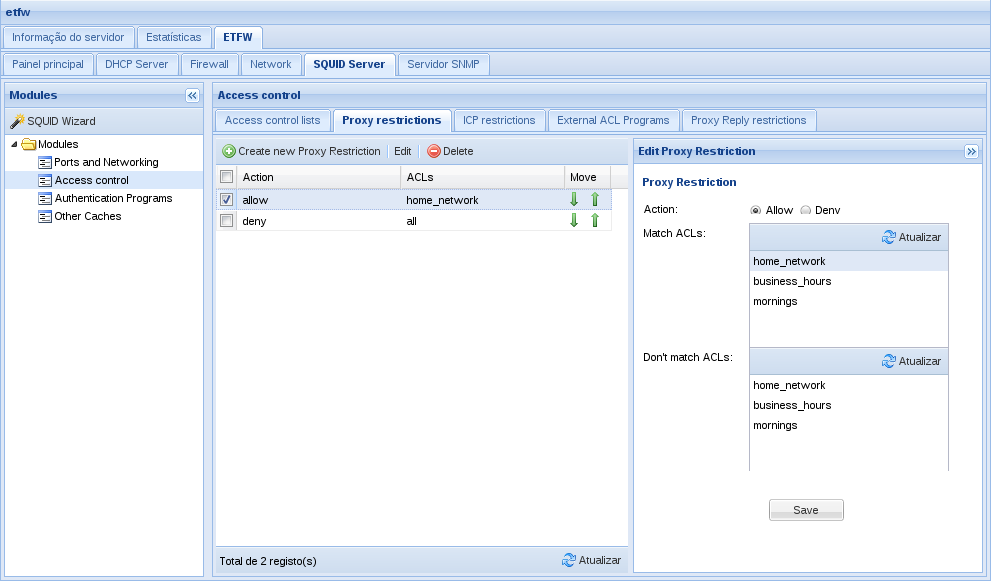
\includegraphics[scale=0.38]{screenshots/etfw/etfw_squid_example_acessoip_02.png}
    \caption{Restringir acessos pelo endereço IP - Criar restrição usando as \textit{ACLs} anteriores}
    \label{fig:etfw_squid_example_acessoip_02}
    \end{center}
\end{figure}

\begin{figure}[H]
    \begin{center}
    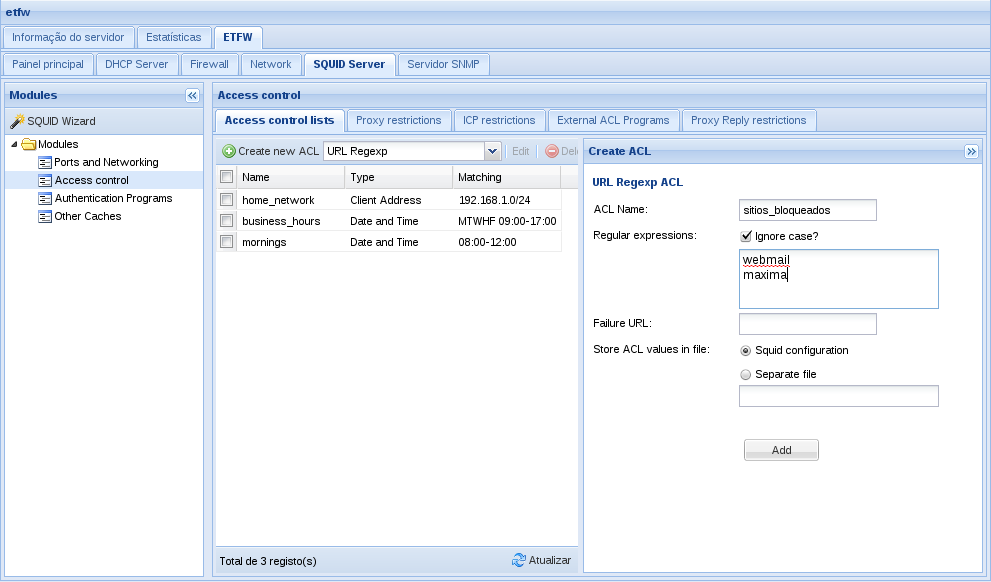
\includegraphics[scale=0.38]{screenshots/etfw/etfw_squid_example_urlregexp_01.png}
    \caption{Negar acesso baseado em RegEXP no URL - Criar \textit{ACLs}}
    \label{fig:etfw_squid_example_urlregexp_01}
    \end{center}
\end{figure}

\begin{figure}[H]
    \begin{center}
    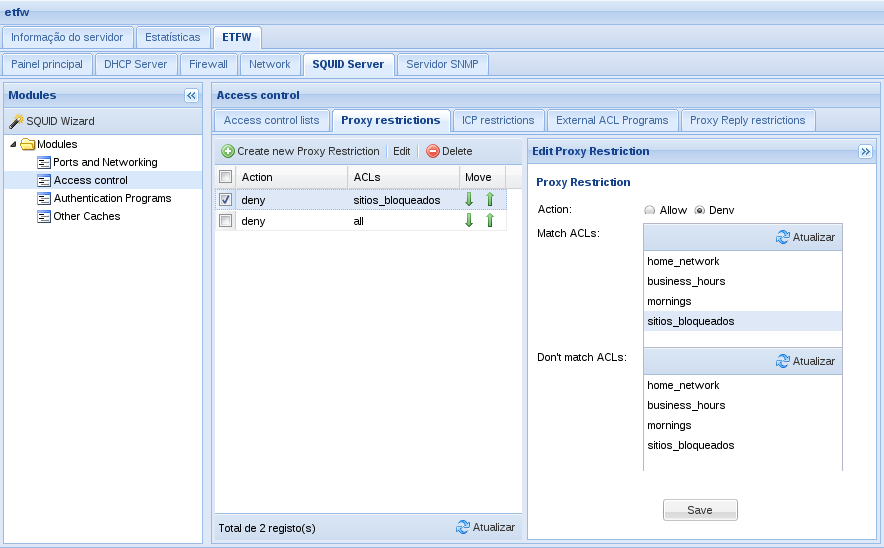
\includegraphics[scale=0.38]{screenshots/etfw/etfw_squid_example_urlregexp_02.png}
    \caption{Negar acesso baseado em RegEXP no URL - Criar restrição usando as \textit{ACLs} anteriores}
    \label{fig:etfw_squid_example_urlregexp_02}
    \end{center}
\end{figure}

\subsection{Servidor \textit{SNMP}}

Na interface de configuração do servidor \textit{SNMP} é possível definir a seguinte configuração:

\begin{itemize}
    \item Informação do sistema: localização e contacto;
    \item IP do servidor de \textit{Trap};
    \item \textit{Community} de \textit{Trap};
    \item Estações de monitorização.
\end{itemize}

\begin{figure}[H]
    \begin{center}
    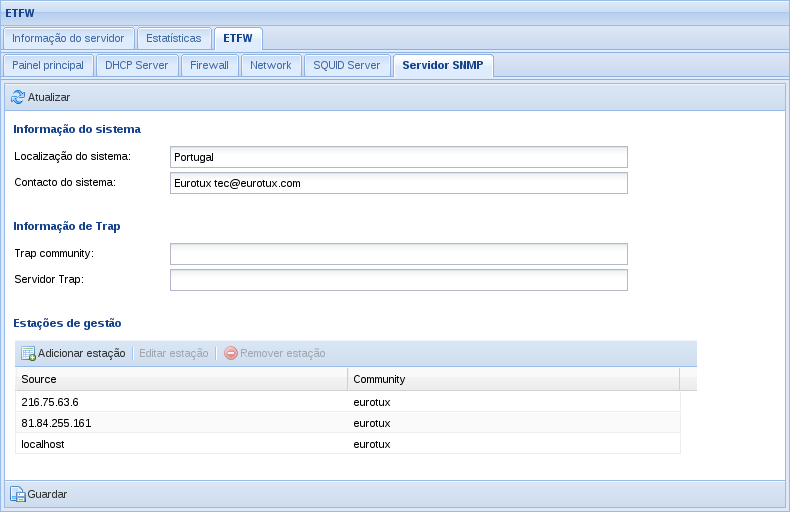
\includegraphics[scale=0.38]{screenshots/etfw/etfw_snmp_01.png}
    \caption{Configuração do servidor SNMP}
    \label{fig:etfw_smp_01}
    \end{center}
\end{figure}

